% Options for packages loaded elsewhere
\PassOptionsToPackage{unicode}{hyperref}
\PassOptionsToPackage{hyphens}{url}
%
\documentclass[
]{book}
\usepackage{amsmath,amssymb}
\usepackage{lmodern}
\usepackage{ifxetex,ifluatex}
\ifnum 0\ifxetex 1\fi\ifluatex 1\fi=0 % if pdftex
  \usepackage[T1]{fontenc}
  \usepackage[utf8]{inputenc}
  \usepackage{textcomp} % provide euro and other symbols
\else % if luatex or xetex
  \usepackage{unicode-math}
  \defaultfontfeatures{Scale=MatchLowercase}
  \defaultfontfeatures[\rmfamily]{Ligatures=TeX,Scale=1}
\fi
% Use upquote if available, for straight quotes in verbatim environments
\IfFileExists{upquote.sty}{\usepackage{upquote}}{}
\IfFileExists{microtype.sty}{% use microtype if available
  \usepackage[]{microtype}
  \UseMicrotypeSet[protrusion]{basicmath} % disable protrusion for tt fonts
}{}
\makeatletter
\@ifundefined{KOMAClassName}{% if non-KOMA class
  \IfFileExists{parskip.sty}{%
    \usepackage{parskip}
  }{% else
    \setlength{\parindent}{0pt}
    \setlength{\parskip}{6pt plus 2pt minus 1pt}}
}{% if KOMA class
  \KOMAoptions{parskip=half}}
\makeatother
\usepackage{xcolor}
\IfFileExists{xurl.sty}{\usepackage{xurl}}{} % add URL line breaks if available
\IfFileExists{bookmark.sty}{\usepackage{bookmark}}{\usepackage{hyperref}}
\hypersetup{
  pdftitle={Two Different Experimental Approches For Testing Temptation And A Test Of Stability Of Individual Risk Preferences},
  pdfauthor={Bettega Paul},
  hidelinks,
  pdfcreator={LaTeX via pandoc}}
\urlstyle{same} % disable monospaced font for URLs
\usepackage{longtable,booktabs,array}
\usepackage{calc} % for calculating minipage widths
% Correct order of tables after \paragraph or \subparagraph
\usepackage{etoolbox}
\makeatletter
\patchcmd\longtable{\par}{\if@noskipsec\mbox{}\fi\par}{}{}
\makeatother
% Allow footnotes in longtable head/foot
\IfFileExists{footnotehyper.sty}{\usepackage{footnotehyper}}{\usepackage{footnote}}
\makesavenoteenv{longtable}
\usepackage{graphicx}
\makeatletter
\def\maxwidth{\ifdim\Gin@nat@width>\linewidth\linewidth\else\Gin@nat@width\fi}
\def\maxheight{\ifdim\Gin@nat@height>\textheight\textheight\else\Gin@nat@height\fi}
\makeatother
% Scale images if necessary, so that they will not overflow the page
% margins by default, and it is still possible to overwrite the defaults
% using explicit options in \includegraphics[width, height, ...]{}
\setkeys{Gin}{width=\maxwidth,height=\maxheight,keepaspectratio}
% Set default figure placement to htbp
\makeatletter
\def\fps@figure{htbp}
\makeatother
\setlength{\emergencystretch}{3em} % prevent overfull lines
\providecommand{\tightlist}{%
  \setlength{\itemsep}{0pt}\setlength{\parskip}{0pt}}
\setcounter{secnumdepth}{5}
\usepackage{booktabs}
\usepackage{booktabs}
\usepackage{longtable}
\usepackage{array}
\usepackage{multirow}
\usepackage{wrapfig}
\usepackage{float}
\usepackage{colortbl}
\usepackage{pdflscape}
\usepackage{tabu}
\usepackage{threeparttable}
\usepackage{threeparttablex}
\usepackage[normalem]{ulem}
\usepackage{makecell}
\usepackage{xcolor}
\ifluatex
  \usepackage{selnolig}  % disable illegal ligatures
\fi
\usepackage[]{natbib}
\bibliographystyle{plainnat}
\newlength{\cslhangindent}
\setlength{\cslhangindent}{1.5em}
\newlength{\csllabelwidth}
\setlength{\csllabelwidth}{3em}
\newenvironment{CSLReferences}[2] % #1 hanging-ident, #2 entry spacing
 {% don't indent paragraphs
  \setlength{\parindent}{0pt}
  % turn on hanging indent if param 1 is 1
  \ifodd #1 \everypar{\setlength{\hangindent}{\cslhangindent}}\ignorespaces\fi
  % set entry spacing
  \ifnum #2 > 0
  \setlength{\parskip}{#2\baselineskip}
  \fi
 }%
 {}
\usepackage{calc}
\newcommand{\CSLBlock}[1]{#1\hfill\break}
\newcommand{\CSLLeftMargin}[1]{\parbox[t]{\csllabelwidth}{#1}}
\newcommand{\CSLRightInline}[1]{\parbox[t]{\linewidth - \csllabelwidth}{#1}\break}
\newcommand{\CSLIndent}[1]{\hspace{\cslhangindent}#1}

\title{Two Different Experimental Approches For Testing Temptation And A Test Of Stability Of Individual Risk Preferences}
\author{Bettega Paul}
\date{2021-12-10}

\begin{document}
\maketitle

{
\setcounter{tocdepth}{1}
\tableofcontents
}
\hypertarget{intro1}{%
\chapter{Introduction}\label{intro1}}

In this thesis, we try to provide elements to test temptation models in the
laboratory.
By temptation model we mean here the model proposed in \citet{gul2001temptation} and
the models inspired by it, like \citet{noor2010uphill} or \citet{noor2015menu}.
Specifically, we are interested in models with the following two characteristics:
They model preferences for menus, that is, preferences for sets of choices in
which only one alternative can be chosen.\footnote{More technicaly menus are subset of the set \(\Delta\) endow with the weak
  topology.
  Where \(\Delta\) is the set of all measures on the Borel \(\sigma\)-algebra of \(Z\) a
  compact metric space \((Z,d)\) of all prizes.}

This approach was initiated by \citet{kreps1979representation}.
And this models must allow preference for the restrictions, that is to say that
an individual can prefer a menu to a menu which is his super set
(i.e to prefer a menu containing less elements).

We are interested in this model because it allows us to rationalize behavior
that cannot be rationalized within expected utility theory.
For example, the demand for a costly commitment \citep{bryan2010commitment, ashraf2006tying}, the exercise of self-control \citep{dellavigna2004contract} or the choice of subscriptions inconsistent with the use of a service \citep{dellavigna2006paying}.
We chose to focus on the temptation model from an experimental point of view
because the theoretical literature already proposes a large number of models
(the reader who wants to be convinced can consult the literature review on the subject \citet{lipman2013temptation}), but the experimental literature on the subject does not propose a design allowing to compare these models;
Both in terms of their descriptive and predictive performance and in terms of their accuracy in describing behavioral frequencies such as the exercise of self-control or the willingness to pay for a commitment.
The experimental literature on temptation is focused on the demonstration of existence of
behavior predicted by theoretical models of temptation and in contradiction with
the expected utility model.
To mention only a few of these works, the exercise of self-control and the costs
it induces first by \citet{mischel1989delay} and then in \citet{kuhn2014self}, the preference for a
restricted set of choices in \citet{toussaert2018eliciting} and the demand for an expensive
commitment in \citet{houser2018temptation}.
This leaves room for an experimental design that would allow us to measure the
effects of temptation on preferences and thus differentiate the different
temptation models.
I therefore propose an experiment to test the descriptive capacity of different
temptation models.

This thesis is composed of three chapters, each describing an online experiment.
The first two experiments aim at testing temptation models, the first one
focusing on a behavioral aspect through the effect of commitment on risk taking.
The second one tests the descriptive capacity of temptation models by eliciting
preferences for menus.
The last one does not test temptation but the stability of preferences for money.
The latter highlights that the instability of individual preferences has
important consequences on the tools used in experimental economics to test a
theory and on the reliability of the preferences elicited.

The original title of this thesis was ``Temptation and strategic interaction:
theory and experiment''.
The objective was to propose an extension to the existing temptation model,
notably those of \citet{gul2001temptation} and \citet{fudenberg2006dual}, to take into account the combined effects of temptation and strategic interactions.
The original PhD thesis project was based on work carried out for my master thesis.
My master thesis consisted in a model that adapted the \citet{fudenberg2006dual} model for two individuals, each composed of two selves and having to decide on the distribution of a budget where their choice
are strategic substitute.
The model developed for the master thesis highlighted that with strategic substitute choice, the
individual with the lowest self-control costs must compensate for the lack of
self-control of the other individual.

My first original work within the scope of this original plan was to propose an experiment to test the
behavioral predictions of the model developed in my master's thesis.
For that I realized a small experiment (40 subjects) built on the experimental design used by \citet{houser2018temptation}.
In this first experiment we tested the self-control capacity of the subjects by asking
them to perform a boring, paid task (looking at a screen displaying the current time) and giving them the possibility to switch to a more interesting, but unpaid task (surfing the
internet).
The subjects were also given the opportunity to costly commit: they could give up a small part of their earnings to continue the boring task without being offered the choice of switching task.
My experimental design consisted of two parts.
The first part was a replication of the \citet{houser2018temptation} experiment and aimed at estimating the individual self-control capacity of the subjects.
The second part aimed at testing their self-control capacity in a context with strategic interactions.
For this purpose, the remuneration of the daunting task was modified to place
pairs of subjects in a situation where their choice are strategic substitute.
The -- ex-ante unexpected -- results of this experiment are that all of our subjects chose to keep performing the
boring task during the 2 hours of our experiment.
This did not replicate the results of \citet{houser2018temptation} who found that
28.7\% of the subjects keep performing the tasks without paying to avoid
temptations and, crucially, did not allow us to test the influence of strategic
interactions.
The differences in results with \citet{houser2018temptation} can be explained by the
differences in dates between the 2 experiments, the original experiment having
taken place in the early 2010s and mine in late 2018.
The relationship to the internet has strongly evolved between these two dates
(think of the actual use of smartphone for example)
and makes an activity like surfing the internet in a lab much less attractive.
This first experiment taught me two lessons that were then applied in the
remainder of the thesis.
First, the choice of the
tempting alternative is difficult because its tempting nature can vary between
individuals but also over time.
making direct replications of past successful design far from trivial.
Second, to test the impact of strategic interactions it would be easier to have
an experimental protocol that does not rely on binary choices but allows for
greater variability in individual behavior.

I therefore started to work on an experimental design, which would give rise to
\protect\hyperlink{tempting-lab}{chapter 3},
that would allow the measure the effect of temptation at the
individual level and which does not depend on the \emph{a priori} level of temptation generated by an
alternative but which allows us to identify which are the alternatives that the
subject considers tempting.
In order to do this, I chose to construct the experimental design in such a way
as to be as close as possible to the theoretical framework proposed by
\citet{gul2001temptation}.
This allow to directly elicit individual preferences for menus, and to build the
menus in such a way as that they induce different level of the temptation
according to different theory.

In parallel to the preparation of this protocol, Rustam Romaniuc and Dimitri
Dubois offered me through Paolo Crosetto the opportunity to propose a treatment
concerning temptation in their experimental project on risk.
Their project planned to measure risk preferences repeatedly before and after an
intervention.
I proposed to test the impact of a freely chosen limit on the maximum level of
risk a player could take.
The intervention consisted in proposing to the subjects to limit the level of
risk they could take in the second half of the experiment and to let them choose
this level.
But with the particularity that this limit would only be applied to a quarter of
the people who would ask for it.
This allows us to observe the limit that subjects desire as well as their
behavior when this limit is not applied.
This allows us to relate the level of the requested limit to the capacity for
self-limitation, from our point of view the link between demand for commitment
and capacity for self-control.
This treatment also allows us to compare the impact of the limit when it is
binding or not.

While analyzing the data from this experiment I noticed an unexpected
difficulty.
I had five observations of risk preferences for each of my subjects before and
five after the treatment, but these five observations seemed to be extremely variable.
This variability between the individual observations was also found in the
observations of the subjects of our control group, who was not exposed to any treatment.
However, if there are many experiments which inform us about the average level
of preference for the subject (for example the \citet{lejuez2002evaluation} or
\citet{crosetto2013bomb} to quote only the ones which inspired chapter 3), there is to
our knowledge no article concerning the individual variability of the
measurement of preferences for risk.
Their is works like \citet{ert2017revisiting} that make multiple measure but don't
compute variability or like \citet{wilcox2007predicting} that compute estimation
error but no one to the best of my knowledge compute individual variability.
Individual variability is necessary to judge the quality of the estimates, as
well as to use simulations to calibrate the experiments and to judge the
reliability of the experimental results.
I have therefore realized an experiment to test the variability of risk
preferences which is described in the \protect\hyperlink{multi-choice}{fourth chapter} of this thesis.
This experiment shows that the variability of individual preferences is
large and must be taken into account in the analysis of experimental
results in the domain of risk attitudes
, on the one hand by having as often as possible a
difference-in-difference analysis as other analysis design causes an
underestimation of the risk of the first type, and on the other hand by
recurring as little as possible to individual level estimations.
Finally, in order to take into account the results of chapter 3 I opted for a
difference-in-difference analysis for the first chapter using a Bayesian rather
than a frequentist approach for the estimates to account for individual
variability.
For chapter two I chose to modify the analysis to test the validity of the
temptation models against statistical models in order to have a reference point.

As during these three years of thesis my work deviated from the initial subject,
I chose to rename my thesis \emph{Two Different Experimental Approches For Testing
Temptation And A Test Of Stability Of Individual Risk Preferences}
Indeed, the central point of this thesis is to explore experimental methods to
test temptation.
The last two chapters are attempts to answer technical problems on the subject.
Therefore the approach chosen throughout the thesis is somewhat different from
the usual approach in experimental economics.
I have chosen to use methods inspired by statistics and machine learning;
notably the use as much as possible of training and test samples to control for
overlearning of the models, the use of bootstrap sampling to compare results
over a large number of samples and smooth the results, and comparisons of the
results of our models with reference models in terms of metrics such as Mean
Square Error (MSE).
The use of these methods aimed at focusing our analysis on errors due to our
observation methods, as well as those of the subjects and model errors that are
rarely taken into account in economics as highlighted in \citet{taleb2005fooled}.
This error-centered approach has two objectives, on the one hand to test the
reliability of the models we are studying and the contribution of the
experimental protocols proposed through this thesis.
On the other hand, it allows us to approach the models we study with a
refutation objective inspired by \citet{popper2005logic} and \citet{popper2014conjectures}.
We compare here the models with dummy models and we show that these dummy models
are better descriptors of individual behaviors.
Of course this method is far from allowing a formal refutation of the models, but it is the
closest method to refutation that I could propose.
The disadvantage of this approach is that it implies focusing on models chosen
specifically in advance and constructing the experiment in such a way as to have
a training set as well as a test set for the model.
The approach chosen as well as the initial objective of answering a technical
problem such as measuring temptation places me in a situation where the links
with the existing literature are limited. This is particularly true with regard to chapter
three, which deals with a question that to best of my knowledge has not been directly studied.

Even if this thesis raises more problems than it answers, I think it brings the
following elements:

\begin{enumerate}
\def\labelenumi{\arabic{enumi}.}
\tightlist
\item
  The first chapter provides new information on the differences between hard
  and soft commitment.
  It allows to put forward a form of complementarity between these two forms of
  commitment.
  This chapter also highlights the way in which subjects choose to use their
  self-control by allowing themselves to exceed their limit at times but by
  reducing their risk-taking below this limit at other times.
\item
  The second chapter shows that taking into account the effect of temptation
  marginally improves the standard model but that these models are not better
  descriptors of subjects' choices on menus than a constant choice model.
\item
  The third chapter highlights that individual choices in the risk domain are
  very variable to such an extent that it does not seem to be described correctly
  by a distribution with a central moment.
  This puts into question both the expected utility model and most random models
  such as \citet{gul2006random}, \citet{ratcliff2008diffusion} or \citet{cerreia2019deliberately}.
  This chapter also highlights a ghost treatment effect, finding significant
  differences between similar groups.
\end{enumerate}

Finally, while this thesis does not propose an experimental protocol for
measuring temptation, it does highlight problems in temptation models as well as
in the expected utility model that invite us to further explore the variability
of individual preferences.

\hypertarget{fdj}{%
\chapter{Intra-personal conflict and self-commitment: Evidence from a sample of French gamblers}\label{fdj}}

\hypertarget{intro2}{%
\section{Introduction}\label{intro2}}

Self control is an important non-cognitive skill that is associated with
favorable economic and social outcomes
\citep{laibson1998self, heckman2006effects, alan2015patience}.
However, abundant evidence suggests that people have a hard time controlling
their instantaneous passions and often succumb to temptation \citep{milkman2021film}.
Consider the two-pack a day cigarette smoker who went through many attempts to
quit but was never successful in kicking the habit.
In New Year's resolutions, one intends to eat more healthy foods in the future,
exercise more regularly, and watch television less often, but many of these
intentions fail because of self-control problems.
One popular solution to self-control problems is to use a commitment device.
For example, in ``How to get ready for retirement: Save, save, save'',
\citet{rankin1993get} suggests to ``Use whatever means possible to remove a set amount
of money from your bank account each month before you have a chance to spend
it.''\footnote{See Deborah M. Rankin, ``How to get ready for retirement: Save, save, save'', New York Times, March 13, 1993, p.~33.}

There is ample empirical evidence showing that hard commitments work well to
reduce one's tendency to err -- as judged by the person's own standards -- in
the direction of instantaneous gratification.
For instance, it has been shown that some people use specific ordering
strategies that enforce watching ``high brow'' movies \citep{read1999mixing}
or that some individuals accept to put their money in temporarily locked savings accounts in order to keep it away from themselves (for more examples, see \citet{milkman2021film}).
Hard commitments allow individuals to ``bind'' themselves as Ulysses did before
setting out to the Syrens \citep{elster2000ulysses}.
However, people often avoid using hard commitments because of their lack of
flexibility.
This is why in the \citet{ashraf2006tying} study that offered customers to commit to
restrict access to their savings, only 28\% accepted the offer and opened a
locked bank account.

An alternative to hard commitments that can work to avoid succumbing to
temptation while providing more flexibility are soft commitment devices, i.e.,
commitments that can be easily broken (See \citet{bryan2010commitment}, for an
extensive review of the literature on commitment devices).
Deviating from soft commitments involves psychological costs such as shame (if
the commitment was made public) or guilt (if it was made privately) or some
degree of both shame and guilt.
Examples of soft commitments backed by non-pecuniary costs include taking a
fixed amount of money when going out with friends (one can always borrow on the
spot, so the commitment is soft), brushing one's teeth earlier in the evening to
avoid late night snacking (the cost of redoing it is low), renting a place in an
open space to avoid taking a nap when working from home (couches may also be
available in open spaces).
Given the ubiquity of soft commitment devices, it is important to understand to
what extent making a commitment soft as compared to hard/binding changes
people's behavior.
However, to our knowledge, there is no empirical evidence on the effects of
soft commitments relative to a condition where the commitment is hard as well as
compared to an environment without any form of commitment device.
Our aim in this paper is to fill this gap.

To study the comparative effects of soft relative to hard and no commitments, we
designed a controlled experiment that we implemented online.
Our sample of 1527 participants who, in the last 12 months prior to their
participation in our experiment, engaged in some sort of legal gambling with
\emph{la Française des Jeux}, the operator of France's national lottery games, with
whom we partnered for this study.
Specifically, our sample is representative of \emph{la Française des Jeux}'s gamblers.
In that sense, this is the first study on self-control that uses such a large
sample of participants and that are representative of the population of gamblers
of a major national operator of lottery games.\footnote{While there are field studies on self control that employ a non-student
  population \citep{ashraf2006tying, milkman2014holding} ,
  we are not aware of any online study on the topic of temptation and self-control
  using a sample of participants with similar characteristics to our participants.}

The experiment consists of two conditions, a \emph{Baseline} that implements a
modified balloon analogue risk task (BART, \citet{lejuez2002evaluation}) and a
\emph{Commitment} condition.
The BART is a risk-elicitation game in which subjects pump air in a fictional
balloon, and collect money proportional to the number of pumps, unless the
balloon bursts, in which case they get no reward.
In the \emph{Commitment} condition, subjects were given the opportunity to select an
upper limit on the number of pumps for future rounds of the BART.
Furthermore, in the \emph{Commitment} condition, subjects are informed that the limit
would be binding with a 25\% chance.
After subjects made their choice regarding the self-imposed limit, they are
informed whether the limit is binding or not.
The fact that the limit is binding with a 25\% chance allows us to capture the
demand for a commitment device as well as to compare decisions under two
different environments:
(1) when commitment is hard given that the limit is binding and
(2) when the commitment is soft given that the subject is free to choose any
number of pumps but knowing that she had committed to limit her behavior to a
certain extent.
Given that the limit has a positive probability of being applied, revealing
one's true preference is a dominant strategy.

We found that 35\% of our subjects ask for a limit to the maximum risk they can
take when offered one.
Asking for this limit has the effect of decreasing the level of risk taken by a
subject, even if this limit is not applied.
The decrease in risk-taking is greater for subjects for whom the limit is
applied, but by studying saturation of the limit as well as the impact of
ex-post application of the limit we show that the effect of accepting the limit
on risk-taking is complementary to the mechanical effect of the limit and not a
substitute.
We can thus see the effects of a hard or soft commitment on risk-taking
behavior.

Our paper relates to the literature that sought to test whether and how
commitment devices can make people succumb less to temptation.
The literature on hard commitment devices has hitherto been considered quite
independently from research that investigates the effects of soft commitments.
For instance, \citet{trope2000counteractive}, \citet{ariely2002procrastination}, and
\citet{houser2018temptation} compare hard commitments to a control without any
commitment.
Despite the importance of such comparisons, a better understanding of hard
commitments requires a comparison between hard and soft devices.
Indeed, hard commitments impose both a pecuniary and a non-pecuniary cost in
case of breach of commitment.
The pecuniary cost can go to infinity if the individual decides to remove
altogether the tempting option from the choice set.
At the same time, hard commitments come also with non-pecuniary costs in case of
a breach such as shame or guilt \citep{kast2014saving}.
The decision to deviate from one's commitment may also signal to the individual
a lack of willpower, which may represent another source of psychological
discomfort \citep{benabou2004willpower}.
On the other hand, soft commitments are backed solely by non-pecuniary costs.
When present, pecuniary costs are mostly symbolic.
Our experimental study allows us to compare the impact of hard commitments
relative to soft and no commitments, thus disentangling the effect of pecuniary
from non-pecuniary costs.

Our work is also related to the theoretical investigation of commitment by
\citet{gul2001temptation}.
In their model, there is a cost of avoiding the most tempting item in a choice
set.
Individuals, therefore, benefit from removing these items.
Our experiment allows subjects to eliminate tempting options from their choice
set by choosing an upper limit on the number of pumps that they will be able to
select.
However, whereas \citet{gul2001temptation} are interested in modelling the demand for
such commitments, we empirically analyze their behavioral effects after some
participants to our study decide to eliminate tempting options from their choice
set.

\hypertarget{mm2}{%
\section{Experimental Design and Procedure}\label{mm2}}

\hypertarget{experimental-conditions}{%
\subsection{Experimental conditions}\label{experimental-conditions}}

Our experiment consists of two experimental conditions: a \emph{Baseline} that
implements a modified balloon analogue risk task (BART, \citet{lejuez2002evaluation})
and a \emph{Commitment} condition where subjects were given the opportunity to select
an upper limit on the number of pumps.

In each condition, subjects played 10 rounds of a modified version of the BART.
The screen showed a small simulated balloon.
Each subject had to choose a number of pumps between 1 and 64, knowing that each
pump would inflate the balloon and would yield a gain of €0.15.
However, each pump could result in the explosion of the balloon.
The probability that a balloon would explode was arranged by constructing an
array of numbers containing the integers 1--64, as in \citet{lejuez2002evaluation}.
The number 1 was designated as indicating a balloon explosion.
On each pump of the balloon, a number was selected without replacement from the
array.
The balloon exploded if the number 1 was selected.
Thus, the probability that the balloon would explode if the subject chose one
pump out of the 64 possible was 1/64.
If the subject chose 20 pumps out of the 64 possible, then the probability that
the balloon would explode was 20/64.
As in \citet{lejuez2002evaluation}, choosing a higher number of pumps
(i) increased the amount to be lost because of an explosion and
(ii) decreased the relative gain of any additional pump.
In our experiment, the average break point was 32 pumps.
That is, a risk-neutral subject would maximize her gains by choosing 32 pumps.

Note that in the original study by \citet{lejuez2002evaluation} subjects had to click
on a pump button to inflate the balloon and they had to click on it as many
times as they wanted knowing that the balloon could explode at any moment.
We modified the original BART study along two dimensions.
First, because we are interested in behaviors under risk rather than ambiguity,
we decided to inform subjects about the range of outcomes and that a priori each
pump is equally likely to result in an explosion.
Second, we asked subjects to choose the desired number of pumps before the
balloon started to inflate.
That is, a subject had to indicate a specific number of pumps and only then the
balloon started to inflate until it reached the chosen number of pumps or
exploded -- whichever happened first.
This way, we did not constrain the number of chosen pumps on balloons that
exploded, which allowed us to capture the subjects' risk preferences in an
unrestricted manner and avoid the truncation of the data that is usual for BART
studies.

In all conditions, at the end of each round, subjects were informed about the
outcome of the balloon task (whether it exploded or not before it reached the
indicated number of pumps) and about their earnings in that particular round.
At the end of the experiment, one round out of the ten was randomly chosen for
payment and this was common knowledge from the outset of the experiment.
The ``pay one'' approach can help to avoid wealth effects and hedging
\citep{charness2016}.

In the \emph{Baseline} condition, subjects played 5 rounds of the BART followed by a 10 seconds
pause where they saw a message informing them that the game would resume after a few seconds.
After the pause, they had to play for 5 more rounds that were identical to the first 5 rounds.
Subjects were informed at the beginning of the experiment that there was a total of 10 rounds.
The 10 seconds pause was implemented to mimic the break that we implemented in the \emph{Commitment} treatment, with the exception of the commitment mechanism introduced in the latter but absent in the \emph{Baseline}.

In the \emph{Commitment} condition, the first 5 rounds were identical to the \emph{Baseline}.
However, at the end of round 5, instead of the pause, subjects were offered the possibility to select an upper limit on the number of pumps that they could choose in all of the rounds that would follow -- i.e., from round 6 to round 10.
All subjects were informed that the limit would be binding with a 25\% chance.\\
For those who opted for no limit, they went on to round 6 of the BART as in the \emph{Baseline}.
For those who opted for a limit, after subjects made their choice, they were informed whether the chosen limit was binding or not.
Then, subjects proceeded to round 6 of the BART.
In case the limit was binding, subjects could choose a number of pumps between 1 and the chosen limit.
If the limit was not binding, subjects could choose any number of pumps between 1 and 64, as in the \emph{Baseline} condition.

Two design choices are worth discussing.
First, the choice of having the first 5 rounds identical across the two conditions.
This sequence was implemented for two reasons:
(i) to allow subjects to get accustomed with the game and
(ii) to capture subjects' ``natural'' risk preferences in the absence of any commitment device.
This way, we can ensure that our subjects have overall similar risk profiles across the two conditions by looking at behaviors in rounds 1-5.
Additionally, we make sure that those who are offered the possibility to choose a limit after round 5 have been exposed to the game and that they had gotten a feeling of their temptation level.

The second design choice that requires a detailed discussion concerns the stochastic aspect of the limit.
The fact that the limit was binding with a 25\% chance allows us to capture the demand for a commitment device as well as subjects' self-control when the limit is effectively implemented (thus, making it a hard commitment) compared to when it is non binding (making it a soft commitment).
Since the limit has a positive probability of being applied, revealing one's true preference is a dominant strategy.
Since it is applied to a minority of subjects only, we can study self-control under a soft and a hard commitment device.

\hypertarget{participants}{%
\subsection{Participants}\label{participants}}

The recruitment process started in October and ended in December 2019.
803 subjects participated in the \emph{Baseline} and 724 in the \emph{Temptation} condition.
Subjects were recruited by a private company, named \emph{Bilendi}, within the framework of a partnership that some of the authors of this study concluded with \emph{la Française des Jeux} (FDJ), which is the operator of France's national lottery games.\footnote{For more information about the two companies, see their respective websites: \href{https://www.fdj.fr/}{FDJ} and \href{https://www.bilendi.fr/}{Bilendi}}

Bilendi recruited subjects for this study from a pool of more than 1 million individuals who had a personal account with FDJ.
The study includes individuals who had declared that they played at least once one of FDJ's games during the 12 months prior to the study (in one of FDJ's physical sale points or online).
Therefore, all our subjects have some appetite for gambling, which makes this
study original compared to using a population that may be less prone to
temptation than the general population.\footnote{For example, Milkman et al.~(2013) study temptation and commitment in a sample of gym users.
  It is quite possible that people who have a gym subscription differ in terms of willpower from people who have no gym subscription.}

The other novelty of our study is that our subjects are more representative of the general population of the country where the study was conducted than the standard subjects included in many experiments that have dealt so far with the topic of temptation and commitment (for example, \citet{ariely2002procrastination}, \citet{casari2009pre}, and \citet{houser2018temptation}, rely on a population of students).

The sample in our experiment was 40.52\% female and 59.48\% male, and relatively more evenly distributed than traditional student samples:
7.50\% of participants were between 18 and 24 years old, 20.67\% between 25 and 34 years old, 37.43\% between 35 and 49 years old, 24.89\% between 50 and 64 years old and 9.51\% were 65 years old or older.
Considering the socio-professional categories, the sample was composed of 46.25\% of CSP- (employee and worker), 26.78\% of CSP+ (farmer, craftsman, merchant, company manager, liberal professions and intermediate professions), 14.05\% of retired or pre-retired, 9.45\% of inactive (not working or looking for a job) and 3.47\% of students.

\hypertarget{control-questions}{%
\subsection{Control questions}\label{control-questions}}

All subjects were recruited by the data collection company \emph{Bilendi}.
Before reading the instructions of the BART, each subject was asked to answer a series of questions about their gambling habits during the last twelve months.
The questionnaire was used to collect information for a different project than the present one.

Additionally, subjects had to answer a series of questions meant to collect socio-demographic information and to check whether they had played one of FDJ's games in the last 12 months (lottery, online poker, and sport betting). Specifically, subjects had to report their gender, age, professional activity, and whether they had bought a lotto ticket, played poker online or made any sport bets within the last twelve months.

At the very end of the BART, subjects were asked to answer 10 questions that correspond to the self-efficacy questionnaire.
This information was collected for a different project than the present one.
The questionnaire was implemented at the end of the experiment and therefore did not influence subjects' risk-taking and commitment decisions.

\hypertarget{procedure}{%
\subsection{Procedure}\label{procedure}}

The online application was developed using the oTree platform \citet{chen2016}.
We created a virtual ``Room'' to generate the URLs and to ensure that each subject would participate only once.
More precisely, the Laboratory for Experimental Economics of Montpellier (LEEM), created a dedicated ``Room'' on its oTree server with identifiers composed of letters and numbers, ranging from A1A1 to Z9Z9.
Consequently, the individual URLs generated by the platform were of the form \url{https://expe.leem.umontpellier/room/leem/?participant_label=A1A1}.
Bilendi, which was in charge of sending the invitations by email, assigned one identifier to each subject, and therefore sent the corresponding URL in the invitation email.
On the LEEM server we only had the identifiers and decisions, while Bilendi had the identifiers and identifying information of the subjects, but did not have access to the decisions of the subjects in the experiment.
This procedure made it possible to guarantee the anonymity of the data collected.
At the end of the experiment, the LEEM sent a file with the identifiers and associated payments to Bilendi, which then paid the subjects via the PayPal platform according to their earnings in the experiment.

The experiment lasted on average 20 minutes and was divided into two parts :
first, the modified BART, with 10 rounds, and then a self-efficacy questionnaire.
Subjects were not informed on the paid round of the BART game until they completed the self-efficacy questionnaire.
The average payoff was €1.60 (std 1.84).
In addition to their earnings related to their decisions, each subject was paid a €5 participation fee.

\hypertarget{result2}{%
\section{Results}\label{result2}}

We proceed to the analysis using 2 sets of data.
The first one corresponds to the baseline treatment and contains the
observations for the 863 subjects who were not subjected to any treatment.
As these subjects simply repeated the elicitation task 10 times, this data
serves as a counterfactual.
The second data set concerns the 724 subjects who were subjected to the temptation treatment.
It is on this data set that our analysis focuses.

For these two data sets we have 10 observations per subject.
But we have chosen not to consider the observations for the first round.
These observations are different from those of the other rounds both in terms of
distribution (evaluated with a Kolmogorov-Smirnov test at a 95\% alpha threshold)
and mean (test of equality of means at a 95\% alpha threshold) for both the
baseline and temptation treatment data.
It is assumed that this is different data because it captures a learning effect.
We therefore apply our analysis to rounds 2 to 10.

For both datasets, we calculated the average before and after treatment for
each type of player.
The results are reported in the table \ref{tab:desc-stat2}.

\begin{table}

\caption{\label{tab:desc-stat2}mean numbers of pumps}
\centering
\begin{tabular}[t]{l|r|r|r|r|r|r}
\hline
 & baseline low type & baseline middle type & baseline hight type & temptation low type & temptation middle type & temptation hight type\\
\hline
before treatment & 21.00 & 21.51 & 21.62 & 21.21 & 18.78 & 23.90\\
\hline
after treatment & 20.65 & 21.06 & 22.90 & 21.08 & 19.99 & 21.28\\
\hline
total & 20.81 & 21.26 & 22.33 & 21.14 & 19.46 & 22.44\\
\hline
\end{tabular}
\end{table}

We can make the following observations:

\begin{enumerate}
\def\labelenumi{\arabic{enumi}.}
\tightlist
\item
  The subjects are globally risk averse with an average number of pumps of
  20.93.
\item
  The high type players are more risk prone than the others but the middle
  and low type players do not differ.
\item
  There is no global difference between the before and after treatment.
  The p-value of the t-test is 0.94 between the pre- and post-treatment
  choices and the p-value for the post-treatment choices between the baseline
  group and the temptation group is 0.4.
\end{enumerate}

Since we cannot reject the hypothesis that the temptation treatment as an effect
on the amount of risk chosen by subjects, we will now look at the choice of
constraint for subjects in the temptation treatment.

To begin with, it is important to remember that the constraint that is proposed
to the subjects in this treatment cannot theoretically serve them to improve
their situation.
Indeed, if the constraint is applied, it only makes the choice of a higher risk
amount impossible.
But even without the constraint, the subjects have no incentive to choose a
higher amount of risk than they want.
Theoretically, we expect subjects not to ask for a constraint.

But we observe that 35\% of the subjects
have asked for a limit.
This quantity is consistent with that observed by \citet{houser2018temptation} (28.6\%
when the limit has no cost) and \citet{toussaert2018eliciting} (35.8\%).
This subject confirms that there is a demand for a constraint in our subjects.
Moreover the limit chosen by the subjects is binding for at least a part of them.
In the table \ref{tab:limit-ask2} we report the number of subjects who requested a limit and
exceeded or reached it before and after it was proposed to them.

\begin{table}

\caption{\label{tab:limit-ask2}share of subject who ask for a limit}
\centering
\begin{tabular}[t]{l|r|r|r|r}
\hline
 & limit exceed before treatment & limit reach before treatment & limit exceed after treatment & limit reach after treatment\\
\hline
limit not apply & 0.41 & 0.25 & 0.3 & 0.31\\
\hline
limit apply & 0.42 & 0.25 & 0.0 & 0.42\\
\hline
\end{tabular}
\end{table}

We see that for 41\% of the subjects the limit that is requested is restrictive
because it is lower than the maximum that was chosen in the first period.
The share of the subjects who reached and exceeded this limit is the same
whether the limit is applied or not before treatment.
On the other hand, the number of subjects who reached their limit without
exceeding it increased after treatment even when the limit was not applied.
This seems to indicate an ability of the subjects to self-constrain.
However, it is interesting to note that the number of subjects who reached or
exceeded their limit remained constant for subjects for whom the limit was not
applied but that this number decreased for subjects for whom it was applied.
This indicates that the application of the limit does not only have the effect
of preventing subjects from taking more than a certain amount of risk.

But our data allow us to go further in the study of the behavior in front of a
constraint.
We can observe not only if the subjects have reached or exceeded the limit but
also to what extent they have moved away from it.
To do this we use a saturation indicator:
\[
r_{saturation} = \frac{pumps}{limit}
\]
And we refer to this inverse as the degree of constraint of the limit.
We will also refer to the truncated saturation ratio which corresponds to the
same ratio but for which the values for which the number of pumps is higher than
the limit are reduced to 1.
This saturated version has the advantage of not being influenced by the
application of the limit and will thus allow us to compare the behaviors of the
subjects for whom the limit has not been applied with those to whom it has been
applied.
The table \ref{tab:sat-ratio2} shows the mean value of the saturation ratio and in parenthesis
the truncated ration value before and after treatment for the subjects who
requested a limit.

\begin{table}

\caption{\label{tab:sat-ratio2}mean saturation ratio (truncated saturation ratio)}
\centering
\begin{tabular}[t]{l|l|l|l}
\hline
 & before treatment & after treatment & difference\\
\hline
limit not apply & 0.89 (0.66) & 0.8 (0.66) & 0.09 (0)\\
\hline
limit apply & 0.83 (0.68) & 0.66 (0.66) & 0.17 (0.02)\\
\hline
\end{tabular}
\end{table}

The following can be observed:

\begin{enumerate}
\def\labelenumi{\arabic{enumi}.}
\tightlist
\item
  The subjects do not saturate their constraint on average.
  Indeed the saturation ratio is less than 1.
\item
  The subjects exceed their constraint when they can, the saturation ratio is
  higher than this truncated value.
  The difference indicates that in terms of the chosen limit, the overshoot is
  important.
\item
  We find the fact that when the limit is applied, the saturation reduction is
  more important.
  But that a reduction is also visible in the subjects for whom the constraint was
  not applied.
\item
  On the other hand, the truncated saturation ratio does not seem to evolve
  before and after treatment whether the limit is applied or not.
\end{enumerate}

We can therefore conclude that choosing a constraint encourages subjects to
self-constrain by reducing their overshoot of the constraint.
But this does not allow us to know if this self-constraint only reduces the
overshoot of the constraint or if it also has an impact for the choices below
the value chosen as limit.

To complete our analysis we studied the impact of proposing a limit, whether it
is accepted and applied, on the level of risk taken by the subjects.
To do this we used the Markov-chain Monte Carlo implementation implemented in
the PyMC package (\citet{salvatier2016probabilistic}).
This method allows us to obtain a distribution for the mean rather than a point
value.
And thus to compare the parameters on their distribution rather than on a
hypothetical normal distribution which turns out to be less precise than the
estimates that we obtained thanks to PyMC.
As MCMC is a Bayesian algorithm, we had to make assumptions on the distribution
of the data and on the associated parameters.
We chose as a prior a Poisson distribution of the data whose parameter is
distributed according to an exponential law with a mean equal to the observed
mean of the data.
The Poisson distribution is justified in that the observed data are discrete,
and for the values of the studied parameters the number of theoretical
observations outside the sample is very low.
Moreover this hypothesis offers better results than the alternative of using a
binomial distribution.

The differences in mean between the before and after treatment periods are
presented in the figure \ref{fig:mean-effect2}.
The differences are compared for 5 different situations.
First in the baseline situation where no differences should be observed between
the first 4 periods and the next 5.
Then in the temptation treatment according to the choice of the subjects when
they were proposed a limit and its consequences.
Finally, we studied what would have happened if the limit they had requested had
been applied to the subject who had requested it but was refused.

\begin{figure}
\centering
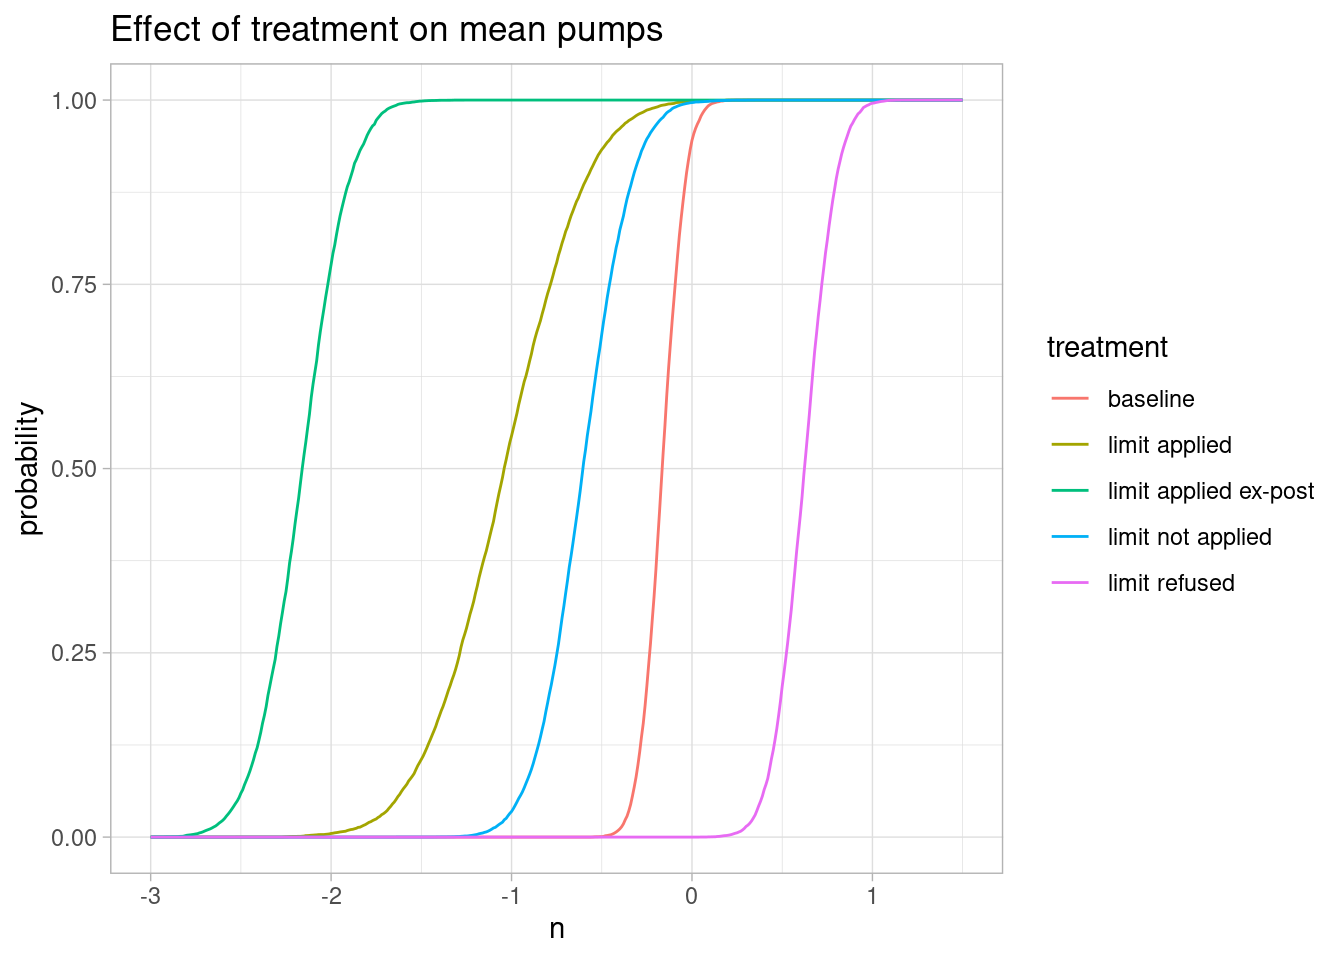
\includegraphics{_main_files/figure-latex/mean-effect2-1.pdf}
\caption{\label{fig:mean-effect2}effect on mean for the different groups}
\end{figure}

We have for the 5 different situations the following estimates in terms of
average difference between the first 4 rounds and the next 5:

\begin{enumerate}
\def\labelenumi{\arabic{enumi}.}
\tightlist
\item
  \emph{limit refused}: mean of 0.63
  with credible interval at 95\% {[}0.34, 0.91{]}.
  We can see that refusing a limit tend to increase the risk taken by subjects.
\item
  \emph{baseline}: mean of -0.17
  with credible interval at 95\% {[}-0.37, 0.04{]}.
  So for baseline their is no significant difference between the four first
  rounds and the subsequent rounds.
\item
  \emph{limit not apply}: mean of -0.61
  with credible interval at 95\% {[}-1.04, -0.17{]}.
  The fact that subjects ask for a limit even if it is not enforced, decreases the
  risk taken by the subjects.
  Although this reduction is small, it is significantly different from what is
  observed for the baseline.
\item
  \emph{limit apply}: mean of -1.03
  with credible interval at 95\% {[}-1.74, -0.32{]}.
  When the limit is applied to the subject who requested it, the average risk
  reduction for subjects is greater than for those to whom the limit was not
  applied.
  However, it is estimated that the probability that the application of the limit
  will result in a greater reduction in the limit is only
  84.54\%.
\item
  \emph{limit apply ex-post}: mean of -2.16
  with credible interval at 95\% {[}-2.58, -1.73{]}).
  The most significant reduction in risk-taking is observed when the limit is
  applied ex-post to subjects who asked for the limit without receiving it.
\end{enumerate}

This analysis of the effect of proposing a limit allows us to complete the
elements mentioned above.
First of all, if the temptation treatment does not create a difference in terms
of risk behavior compared to the baseline, this is due to the fact that even if
the subjects who asked for a limit reduced their risk taking, the subjects who
refused it increased their risk taking.
Second, we show that asking for a limit, even if it is not enforced, leads
subjects to reduce their risk-taking.
This shows that subjects are able to self-constrain.
But this self-constraint does not seem to be as effective as a binding limit
because the reduction in risk-taking is greater when the limit requested by the
subjects is applied.
Finally, we see that the reduction in risk-taking is even greater when the limit
is applied ex-post.
This confirms what we have seen with the saturation of the constraint, that is
to say that the effort of self-constraint to reduce the level of risk taken is
applied by reducing the risk taken below the limit requested but that the
subjects do not seem to succeed in not exceeding their limit by themselves.
This observation is consistent with the idea of convex self-control costs but
this hypothesis will have to be tested by future work.

\hypertarget{discu2}{%
\section{Conclusion}\label{discu2}}

The extant literature has investigated the effects of hard commitment devices,
that impose financial and non-financial costs in case of breach of commitment
(e.g., \citet{ashraf2006tying}) separately from soft mechanisms, such as signing a
pledge, that are backed solely by guilt and discomfort (e.g., \citet{bhanot2017cheap}).
As not everyone is comfortable with the idea of a commitment device that imposes
significant penalties or restricts future freedoms, those who cannot stomach the
thought of hard commitments may do better with a different flavor of commitment
device.
It is, therefore, important to understand to what extent soft commitments are a
good substitute for hard ones.
Our experimental study is the first, to the best of our knowledge, that compared
the impact of a hard commitment device relative to soft and no commitment, thus
disentangling the effect of pecuniary and non-pecuniary costs on one's capacity
to not succumb to temptation.

To study the effects of hard versus soft commitments, including a condition with
no commitment device, in a comparable and controlled environment, we implemented
an online experiment with 1527 participants.
Compared to more standard experiments that examined temptation in the lab, our
subject pool is more diverse in terms of age and occupation (only 7.5\% were
between 18 and 24 years old).
Furthermore, compared to some field experiments (e.g., \citet{ashraf2006tying}), our
study retains the advantages of laboratory studies in terms of control over the
subject's decision environment as we implemented an online balloon analogue risk
task.
Finally, in terms of our subject pool, contrary to some field studies (e.g.,
\citet{milkman2014holding}), our participants are particularly tempted by the activity
that they can choose to limit as we recruited participants a pool of individuals
who have engaged in sort of gambling activity over the last 12 months prior to
the study.
Thus, our experiment can be viewed as an artefactual field experiment, to use
\citet{harrison2004field} taxonomy because we use a standard task with an abstract
framing, but with a nonstandard pool of participants.

Our results demonstrate that there is a demand for constraint in about one third
of the subjects.
The subjects who request this constraint decrease their risk-taking even when
this constraint is not applied.
We see that the decrease in risk-taking is more important in subjects for whom
this constraint is hard.
We have shown that the decrease in risk-taking in subjects for whom the
constraint is soft is different and complementary to the decrease in
risk-taking in subjects for whom the constraint is hard.
This complementarity of behaviors between hard and soft constraints
invites us to explore theoretical models that postulate that individuals are
both requesting constraints and capable of self-constraint.
Among these models, temptation models such as those proposed on the
\citet{gul2001temptation} model allow to rationalize the behaviors highlighted in
this article.
More specifically the model of \citet{noor2015menu} allows to rationalize the
effect of the application of the ex-post limit as well as the non-saturation of
the constraint by subject.

\hypertarget{tempting-lab}{%
\chapter{Descriptive Power of Tempting Model}\label{tempting-lab}}

\hypertarget{intro3}{%
\section{Introduction}\label{intro3}}

In this chapter we present an experiment which aims to test the descriptive
capacity of the model proposed by \citet{gul2001temptation} (hereafter G-P).
The predictions of this model are compared with those of different economic
models and with simple statistical models.
To evaluate the descriptive capacity of the models, our experiment places
subjects in a situation as close as possible to the theoretical framework of
G-P.
Subjects are asked to choose by means of an incentivized elicitation mechanism
among menus composed by lotteries.
A menu here is a set of 1 to 6 lotteries, from which the subject knows that she will have to
choose only one lottery in the end.
Our approach differs from that of the previous chapter and from experiments such
as those of \citet{houser2018temptation} or \citet{toussaert2018eliciting} on the subject.
Our experiment does not aim at showing the existence of a particular behavior
predicted by the theory such as the demand for commitment or the capacity of the
subjects to exercise their self-control.
It aims instead to evaluate the
ability of G-P to describe the actual behavior of the subjects,
and to compare its performance to various alternatives, ranging from economic to
statistical models.

This experiment does not question the existence of behavior at odds with expected utility theory,
such as the demand for constraints (\citet{chow2011demand}, \citet{gine2010put} and \citet{uhl2011self}),\\
self-control effects (\citet{burger2011field}, \citet{mischel1989delay} and
\citet{kuhn2014self}) or more surprising attitude like in
\citet{dellavigna2006paying}.
These behaviors are well established in the experimental literature.
Our experiment questions the menu preference approach as a way to rationalize
these behaviors.
This approach, initiated by \citet{kreps1979representation}, aims at rationalizing the
preference that individuals may have for larger sets of choices.
The idea being that an individual who is uncertain about his future preferences
would prefer to have a larger number of options to choose from when making his
decision in order to maximize his utility.
Later G-P proposed a model in which individuals may be averse to the\\
presence of certain options and therefore prefer smaller choice sets.
G-P's model rationalizes the demand for constraints by subjects while allowing
for the possibility of costly self-constraint.
The G-P model was later extended to rationalize more behaviors.
For example \citet{gul2004self} for repeated choices , \citet{noor2010uphill} for anticipated
temptation cost or \citet{noor2015menu} for more complex interactions among elements of
a menu -- for a review of application and extensions of the original G-P model see the review by
\citet{lipman2013temptation}.

Our experience shows that in terms of descriptive power the G-P model is a
slight improvement over EUT.
But the G-P model does not do better than a model where subjects all evaluate
their menus in the same way and independently of their composition.
Moreover, a simple regression model outperforms the G-P model.

The goal of our design is to be as close as possible to the theoretical
framework formulated by G-P. We have therefore focused on the ellicitation of
the menu value.
Therefore we do not have a mechanism that would allow us to identify the
different states of the world that are at the basis of the temptation models
proposed by \citet{dekel2001representing}, \citet{dekel2007representing} or
\citet{dekel2009temptation}.
Nor can we identify the choices of different selves as in the multiple-self
models proposed by \citet{fudenberg2006dual}.
Therefore, we will not propose any interpretation of our data in the framework
of these models.

Our approach will allow us to propose a method allowing us to elicit the two
functions used in the G-P model for each of our subjects.
G-P shows that an individual whose preferences are complete, transitive,
continuous, independent and satisfying the axiom of \emph{Set Betweenness}:
\[
A \succsim B \text{ implies } A \succsim A\cup B \succsim B
\]
has a utility function for menus of the form:
\[
U(A) = max_{x \in A}(u(x) + v(x)) - max_{y \in A}(v(y))
\]
With \(A\) and \(B\) was menus and \(u(.)\) and \(v(.)\) was Von-Neumann Morgenstren
utility functions.
What we will do in our analysis is to estimate for each menu the value
associated for the function \(u(.)\) and for the function \(v(.)\) and to compare
the theoretical value of the resulting menu to the one indicated by the subject.
We do not test the validity of the axioms but that of their theoretical
consequence.

\hypertarget{mm3}{%
\section{materials and methods}\label{mm3}}

\hypertarget{experimental-design}{%
\subsection{Experimental design}\label{experimental-design}}

Our experience took place from 12/06/2020 to 19/08/2020.
It took place online and the recruitment of the subjects was done via the Amazon
Mechanical Turk (AMT) platform.
On the AMT platform a job offer was published indicating the approximate
duration and the fixed payment as well as an average bonus higher than 5\$.
From this offer, subjects could accept to participate in our experiment by
accepting the task on AMT.
No selection criteria are applied a priori to the subjects. But only the subjects having filled in a valid end-of-experience code were included in the analysis. Conditions of minimum duration of working time and number of trials are also applied but do not exclude any subject \footnote{Only subjects with a valid code are kept because this code allows us to pay the subjects and the author refuses to include subjects who were not paid in the study. The exhaustive inclusion criteria are listed in the pre-registration of the study available with asPredicted code
  \href{https://aspredicted.org/qj8mr.pdf}{qj8mr}}.

The software itself is developed using the R language and the Shiny framework.
Once the experiment is completed, the experimental software displays a summary
of the subjects' bonus and a unique code to be filled in the corresponding field
on the AMT platform.
This code allows us to uniquely identify the subjects' responses between our
software and the AMT platform.
The target number of subjects was 300.
304 subjects filled in a response code on the AMT page but this code was only
valid for 297 of them.
The 7 subjects whose code was not valid were excluded from the dataset and were
not paid.

The experience proceeds
as follows:

\begin{enumerate}
\def\labelenumi{\arabic{enumi}.}
\tightlist
\item
  The subject faces a screen with instructions.
  This screen describes the next steps in the experiment and details how the
  subject will earn his payoff.
  The subject is given a description of the menu and how the lottery works.
  Particular emphasis is put on the impact on the bonus of the mechanism of choice
  of a menu.
\item
  The subject has to answer a short series of multiple-choice control questions.
  To continue, the subject must answer all questions correctly.
  To do so, he has as many attempts as he wants and a help is displayed for the
  questions to which the answer is wrong at the first attempt.
\item
  Start of incentivized learning phase:
\item
  The subject has to bid on 10 pairs of menus by indicating with a slider the
  maximum amount he is willing to pay between -1\$ and 1\$ (the bidding mechanism
  is described in detail in the following section).
  The menus on which the subject bids are built in the same way as those of the
  rest of the experiment but the values used for the lotteries that compose them
  are different.
\item
  One of the bids that has just been made is drawn and the subject chooses one
  of the lotteries that it contains.
\item
  A screen indicates to the subject what amount he has won with the steps 4 and
  5, either the amount resulting from the selected auction and the amount
  corresponding to the resolution of the chosen lottery.
\item
  The subject is asked to complete a second quiz similar to the one in step 2
  but with different questions.
\item
  Main taks: the subject bids on 35 comparisons between 2 menus.
\item
  5 of these comparisons are drawn at random and the subject can choose 1
  lottery from each of the 5 menus assigned to him according to her bid and the elicitation mechanism.
\item
  The lotteries are solved and the subject's bonus is calculated as the total
  won on the 5 bids on the selected comparisons and the results of the 5 chosen
  lotteries plus what was already won in the learning phase.
\item
  On the final page, a table summarizes the subject's winnings by selected
  comparisons indicating the amount won via the auction and the lottery results.
  The total of the 6 auctions and lotteries is also displayed along with a
  reminder that the subject must fill in the code displayed on this page on AMT.
\end{enumerate}

Our experiment is composed of only one treatment.
The earnings of the subjects are paid via the AMT platform.
They are composed of a fixed part of 1\$ paid to all the subjects who filled in
a valid code in the AMT form, and a variable part calculated according to the bids on the 6 selected
comparisons and the resolution of the 6 lotteries they chose (1 in the learning
and 5 in the main phase).

Our subjects were thus paid an average of 6.97\$ for
an average time of 41 seconds spent on our experiment.
So an average wage per hour of
10.3\$

The objective of our experimental protocol is to elicit the value that subjects
place on menus.
A menu is a set of items from which the subject must choose 1 and only 1 item.
To be as close as possible to the theoretical model of G-P we chose to build our
menus with lotteries.
In order to keep our experiment as simple as possible we chose to use binary
lotteries similar to the bets that can be made in roulette games in casinos.
That is to say lotteries allowing to win \(n\)\$ with a probability of \(\frac{1}{n}\)
and 0\$ otherwise.
The menus can be composed of 1 to 6 lotteries with the possible values of \(n \in [2, 4, 6, 8, 16, 32]\).
All lotteries have the same expected value of 1, and differ in variance only, that is increasing in \(n\). This keeps the individual elements of the menus as simple and intuitive as possible.

To elicit the value of the menus we have chosen to use a variant of the BDM auction
method proposed by \citet{becker1964measuring}.
This auction method consists in asking the subjects the maximum amount they
would be willing to pay to acquire a good, then to randomly choose a number;
if the number drawn is lower than the value announced by the subject then the
subject must buy the good for the amount drawn.
This method encourages the subject to reveal the true maximum amount he is willing to
pay for a good.
Indeed, a subject who does not indicate his true value runs the risk of paying
more for a good than he is willing to pay or risks not acquiring the good for an
amount lower than what he would have been willing to pay.
The method we use differs from the one presented in \citet{becker1964measuring} because
we want to compare menus between them.
So we ask subject for the maximum amount he is willing to pay to \emph{exchange} one
menu for another (we will call this amount willingness-to-change, WTC).
So to elicit the WTC between 2 menus we present to subjects the one menu on
the left of the screen and the other on the right, the subject has to indicate an amount
between -\$1 and \$1 corresponding to the maximum amount he is ready to pay to
exchange the menu on the left against the one on the right.
If the randomly chosen number is less than the value indicated by the subject,
the subject receives the right menu and must pay an amount equal to the number
drawn (paying a negative amount means receiving money).
If the number drawn at random is strictly higher than the amount indicated by
the subject, the subject receives the left menu.

In our experiment, subjects indicate the maximum amount they are willing to pay
using a slider located between the 2 menus.
In order not to induce an anchoring effect, the initial position of the slider
is determined randomly for each comparison.
This allows us to see that in 85.39\% of the
cases the subjects have effectively indicated their preference by moving the
slider from the place where it was initially placed.

As with 6 different items it is possible to build 63 different menus and
therefore 1953 different 2-by-2 comparisons, we restricted the comparisons made
by the subjects to the one that seemed the most interesting for us\footnote{In retrospect, knowing the results of the experiment and given the problems found on value
  imputation with a utility function it would have been better to restrict the
  number of items to 4 and thus be able to explore more thoroughly the space of 2-by-2 comparisons.}.
The 35 comparisons that we have retained for each subject are the following:

These comparisons were chosen to allow reliable estimates of preferences with many
observations of comparison of size 1 menus with each other and with size 2
menus;
but also to cover a wide range of items and menu sizes.

\begin{enumerate}
\def\labelenumi{\arabic{enumi}.}
\tightlist
\item
  10 comparisons between menus of size 1.
  The menus of size 1 are chosen randomly but in such a way that each menu appears
  at least once and that it is possible by 2-by-2 comparisons to reconstruct 1
  chain of all menus of size 1.
  This comparisons is used to estimate singletons preferences.
\item
  12 comparisons between menus of size 1 and size 2.
  The menus to be compared are drawn at random but we make sure that the menus of
  size 2 containing the elements 2 and 32 (the extreme lotteries) are compared at
  least once with the menus of \{2\} and \{32\} in order to facilitate the imputation
  by a utility function of the elements which were not directly compared.
  This comparisons is used to estimate temptation preferences
\item
  3 menus of size 2 between them drawn at random.
\item
  3 menus of size 3 with menus of size 2 drawn at random.
\item
  1 menu of size 5 drawn at random with 1 menu of size 4 and 1 menu of size 2.
\item
  menu of sizes 6 with 1 random menu of each other size.
\end{enumerate}

Finally, as the subjects have chosen menus and once all the comparisons are
done, 5 comparisons among the 35 are be drawn at random and a menu for each of
the chosen comparisons is selected using the described procedure.
The subject then have to choose in each of these menus 1 and only 1 lottery.

\hypertarget{estimations-and-models}{%
\subsection{Estimations and Models}\label{estimations-and-models}}

In order to implement the economic models on our data, it is necessary to
estimate the preferences of the subjects. In the following sections we present
the methods we have chosen.
In order to estimate individual preferences on singletons, we use the following
methodology:

\begin{enumerate}
\def\labelenumi{\arabic{enumi}.}
\tightlist
\item
  We consider a menu comparison set of size 1.
  For each comparison we construct 2 equations.
  For example, if we consider the comparison between a menu A and a menu B we
  construct the 2 equations:

  \begin{itemize}
  \tightlist
  \item
    \(A = B + x\)
  \item
    \(B = A - x\)
  \end{itemize}
\item
  We assign a value of 0 to one of the menus.
\item
  We solve each equation for which the right-hand side can be calculated.
\item
  Each singleton is assigned the average value of the equations for which it is
  the left-hand member that could be calculated.
\item
  Repeat step 3 until the desired number of iterations is reached.
\item
  Each singleton is assigned the average value of the last n iterations (or n
  an arbitrary number).
\item
  We normalize the values by subtracting the value of one of the singletons.
\end{enumerate}

We tested this methodology on our data and the procedure seem to converges
quickly after about 30 iterations the variation in the estimated value is
negligible.
And the result is independent of the singleton chosen as starting point.

This methodology allows us to estimate the preferences for the singletons while
taking into account the variability in the subjects' responses.
However, this method is based on 2 assumptions.
The first one is that there is indeed a preference value for the singletons to
be estimated and the second one is that the comparison of elements is
symmetrical.
We do not test either of these two hypotheses in our experiment but consider
them as valid or at least as reasonable approximations.

To estimate the effect of temptation, we use a procedure similar to the one used
to estimate preferences for singletons.
The only difference is the way we build the equations from a comparison between
2 menus.
As an example, we focus here on comparisons between menus of size 2 and size 1.
We use the estimates made on the singletons to identify the preferred item in
each menu of size 2, once this item is identified we compute a theoretical
difference with the menu of size 1 by subtracting the estimated value of the
preferred item of the menu of size 2 from the one of size 1.
We calculate the corrected comparison of preferences that we use to build our 2
equations.
For example let's consider the comparison between the menus \(A = \{a_1, a_2\}\)
and \(B = \{b\}\), and suppose that the estimates of the preferences for the singletons yield \(hat{u}(\{a_1\}) > \hat{u}(\{a_2\})\).
We note \(wtc_t = \hat{u}(\{a_1\}) - \hat{u}(\{b\})\).
We construct the 2 equations:

\begin{itemize}
\tightlist
\item
  \(A = B + x - wtc_t\)
\item
  \(B = A - x + wtc_t\)
\end{itemize}

With these equations we use the same procedure as for the estimation of
singletons.
The preferences estimated in this way allow us to calculate the value predicted
by the expected utility model for each of our 35 menus.

In our analysis we will compare the results of 5 different models.
These models are grouped in two categories, the statistical models which are the
application of statistical methods to our data and the economic models which are
implementations of economic theories adapted to our data.
The two statistical models are the following:

\begin{enumerate}
\def\labelenumi{\arabic{enumi}.}
\item
  Constant response model.
  This model consists in calculating for each individual the aggregate average WTC he is
  willing to pay, over all comparisons between menus of size one and between menus
  of sizes two and one.
  This model predicts that the WTC of an individual for any pair of menu items is
  his average aggregate WTC.
  This model is dummy but it is useful as a lower-bar reference point. It seems reasonable to assume that a relevant model is more efficient than this constant response model.
  Using this kind of dummy model as a comparison point is a common practice in
  machine learning.
\item
  Linear regression.
  This model consists in estimate a linear regression model for each individual.
  The explained variable of this regression is the WTC between 2 menus and the
  explanatory variables are variables indicating the presence of the elements in
  the compared menus.
  This type of model is the usual starting point in machine learning, it is
  relatively simple, not expensive in terms of calculation and can easily predict
  new values if we have the corresponding explanatory variables, which is our
  case.
\end{enumerate}

The economic models that we have chosen are the following:

\begin{enumerate}
\def\labelenumi{\arabic{enumi}.}
\item
  The expected utility model (EUT).
  This is the model that corresponds to the \emph{standard theory} in economics where
  the value of a menu depends only on the value of the item inside it that will be
  chosen, therefore on the preferred item that it contains.
  We have chosen to call it the expected utility model because our menus contain
  lotteries.
  The WTC between two menus is calculated as the difference between the preferred
  items that each menu contains.
  We have to estimate for each individual the relative value of each item
  contained in the menus.
\item
  The Gul and Pesendorfer model (G-P).
  In this model, we estimate the value of a menu with the following formula:
  \[ U(A) = max_{x \in A}(u(x) + v(x)) - max_{y \in A}(v(y)) \]
  We have to estimate for each individual two preferences for each item present in
  the menus.
  and we estimate the WTC as the difference between the estimated values of the two
  menus.
\item
  The cumulative temptation model.
\end{enumerate}

We estimate the value with the following formula:
\[ U(A) = max_{x \in A}(u(x) + v(x)) - \sum_{y \in A}(v(y)) \]
This model uses the same estimation as the previous one but this time the
temptation effect of all the items of a menu is taken into account not only the
one of a particular item.

\hypertarget{result3}{%
\section{Results}\label{result3}}

Our analysis is based on the assumption (that we don't test) of symmetry of the
WTC.
Indeed, we consider that if an individual is willing to pay x\$ to switch from
menu A to menu B, this individual will be willing to pay -x\$ to switch from
menu B to menu A.
As we consider this hypothesis to be true, we applied it as a pre-processing on
our data so that the left menu is always the larger of the two menus to compare
by modifying the WTC multiplying it by -1 when necessary.
This modification is intended to make the analysis easier to understand and does
not change the results.

The starting point for estimating the different economic models presented is the
estimation of individual preferences.
We will then estimate the preferences of each individual by following the method
explained.
To estimate the preferences on the singletons we use the 10 comparisons of menus
of size 1 made for each individual.
We iterate on the resulting equation system 500 times and we keep as value for
each item the average of the last 50 iterations.
Finally as we compute relative preferences, we normalize each value by
subtracting the value of the singleton \{2\}.
This method gives us estimates for the 6 possible singletons for
98.32\% of our subjects.
An error in the programming of the experimental software has wrongly validated
strings of singletons for 1.68\% of the subjects making our
estimation procedure invalid for them, so we have removed these subjects from
our study.

Since singletons can be seen as lotteries, we can test if subjects have
consistent preferences in terms of risks.
We consider preferences as consistent in terms of risk if the singleton \{N\} is
the singleton whose estimated utility is maximum then the estimated utility of
the singleton \{P\} is higher than that of the singleton \{Q\} if \(N > P > Q\) or if
\(N < P < Q\) i.e.~single-peaked preference.

Among our subjects we find that
10.27\% have consistent, single-peaked
preferences.
This may seem low and could call into question our method of estimating
preferences.
However, our estimates are strongly correlated with the subjects' responses as
presented in the figure \ref{fig:uEstim-plot3}.
The small number of subjects with single-peak preferences combined with the
elements presented in the next chapter concerning the difficulties of estimating
individual utility functions leads us not to try to smooth values in our
estimates.
An erroneous smoothing could be harmful to our analysis.
If this does not pose a major problem in the case of the estimation of
singletons, we will see that it is on the other hand problematic for the
estimation of the temptation effect.

\begin{figure}
\centering
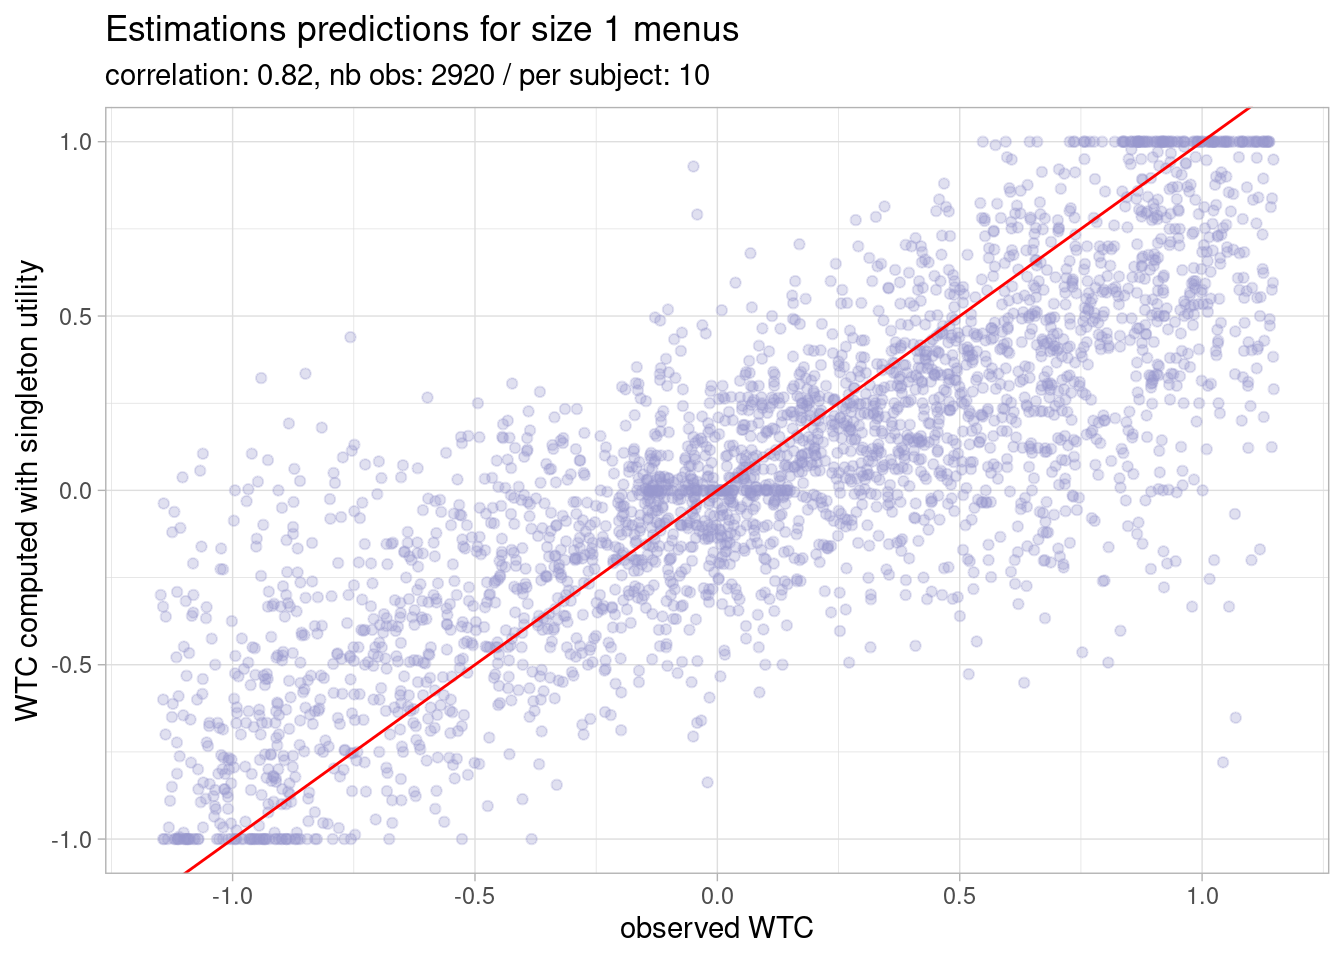
\includegraphics{_main_files/figure-latex/uEstim-plot3-1.pdf}
\caption{\label{fig:uEstim-plot3}High correlation between observation and estimation WTC for size 1 menus}
\end{figure}

Using the estimated utilities for the singletons and the 12 comparisons between
size 2 and size 1 menus we can estimate the temptation utility of each item for
each subject.
We iterate again 500 times on the equation system provided by the 12 comparisons
and we retain for the estimation of the relative utility of each item the
average of the last 50 iterations.
To normalize we substract to all value the estimate for the temptation element
\(2\).
We obtain estimates for each subject, but as foreseen by our design, we do not
have the estimates for each item.
The table \ref{tab:no-estim3} summarizes the percentage of subjects for whom we have no
estimate by item.

\begin{table}

\caption{\label{tab:no-estim3}Share of subjects without estimation by items}
\centering
\begin{tabular}[t]{r|r|r|r|r|r}
\hline
2 & 4 & 6 & 8 & 16 & 32\\
\hline
0 & 15.75 & 19.18 & 15.75 & 13.7 & 0\\
\hline
\end{tabular}
\end{table}

With 37.67\% of the subjects for whom 1 item has no
estimate and 13.36\% for whom 2 items have no estimate.
As these missing estimates are not located on the extreme values, theoretically
it would have been easy to impute them by smoothing the estimated values with a
utility function.
But we have seen with the estimates of the singletons that such a smoothing is
not reasonable in practice, as the level of consistency is too low to make this
a meaningful exercise.
We will therefore keep this value as missing in the rest of the analysis.
But missing values do not seem to have an
important impact on the predictions of the G-P model.
Indeed, by comparing the predictions made on all the comparisons between menus
the correlation between prediction and observation is
0.45 on all the available
value and
0.47
when we restrict on observation for which we have all item estimated.
Since restriction to full estimate item menus don't seem to have an important
impact in the analysis, in the following we willuse all available data.
The figure \ref{fig:pref-estim-plot3} shows the distribution of the estimates
for each of the items.

\begin{figure}
\centering
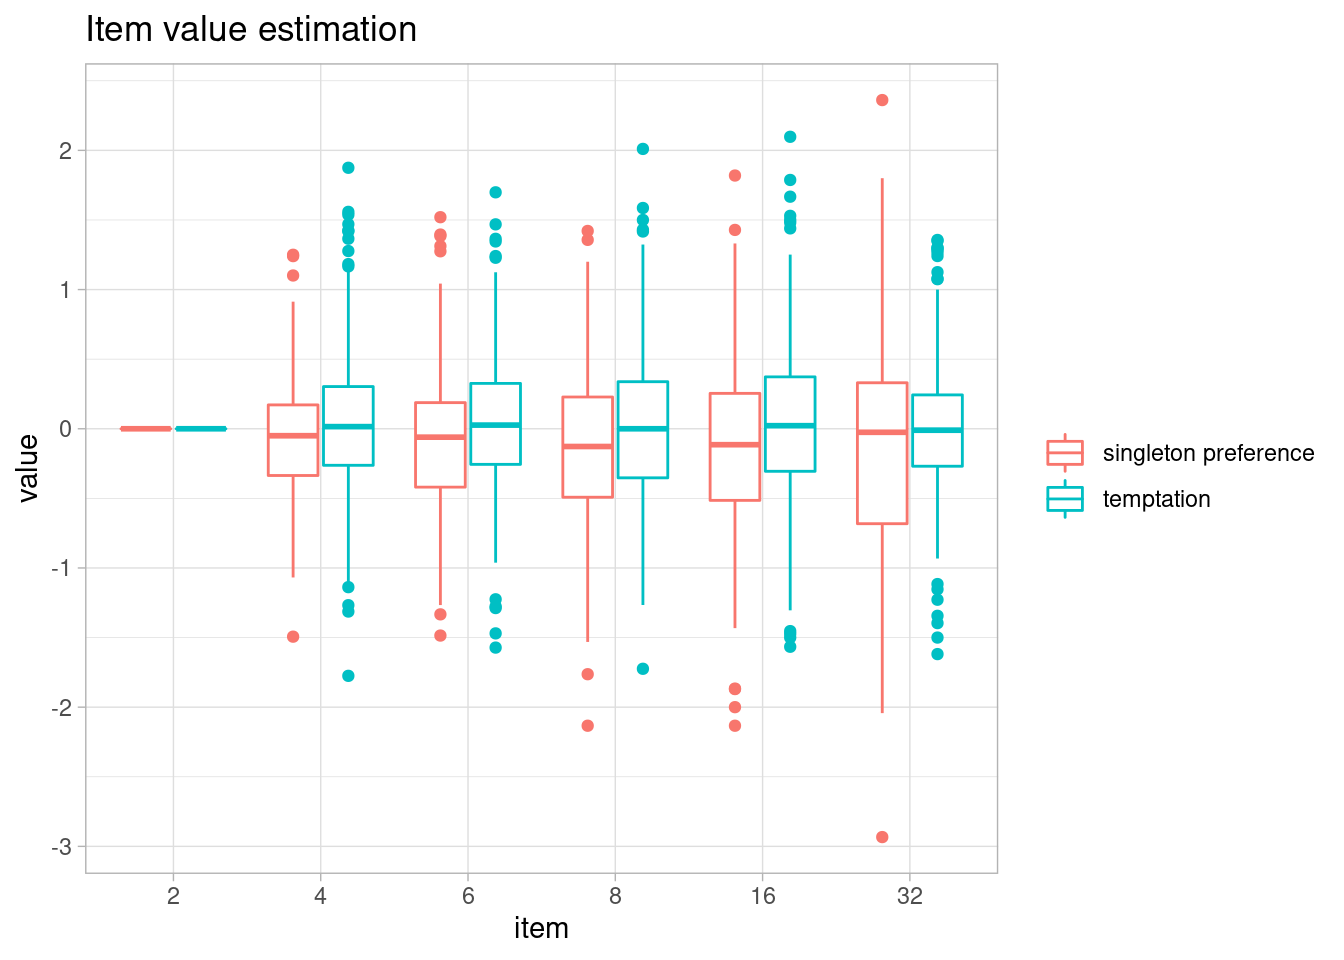
\includegraphics{_main_files/figure-latex/pref-estim-plot3-1.pdf}
\caption{\label{fig:pref-estim-plot3}Distribution of the estimate value of item for all subjects}
\end{figure}

We can see that the estimates are of the same order of magnitude across items
and across preferences for singletons and for the temptation effect.
The estimates for singletons seem slightly lower than for temptation but this
does not seem to be a significant difference.
There are no elements that appear to be outliers in these estimates.
Using these estimates we can calculate for each of our economic models the WTC
of each comparison made by our subjects.

As a comparison tool to judge the quality of the predictions of our models we
estimate two statistical models, a constant response model and a regression
model.
To estimate the constant response model, we simply compute the average of the
subjects' responses in terms of WTC for the size 1 menu comparison and for the
comparison between size 2 and size 1 menus.
The average of these 22 comparisons for each subject is the prediction for any
comparison made by this model.

The regression model is estimated as follows.
For each subject, a linear least square regression model is estimated with the
data concerning the size 1 menu comparisons and the size 2 menu comparisons with
size 1 menu.
The model has the following form:

\[
WTC = \beta_0 + \beta_1 L_2 + \beta_2 L_4 + \beta_3 L_6 + \beta_4 L_8 + 
\beta_5 L_{16} + \beta_6 L_{32} + 
\beta_7 S_2 + \beta_8 S_4 + \beta_9 S_6 + \beta_{10} S_8 + \beta_{11} S_{16}
\]

Where \(L_i\) is an indicator variable for the presence of item \(i\) in the largest
menu and \(S_i\) the same for the presence of \(i\) in the smallest menu.
Note that our model does not contain the indicator variable \(S_{32}\) because it
is a linear combination of the other variables given the menu size constraint.
The estimates of each of the model parameters for each subject are shown in the
figure \ref{fig:reg-estim-plot3}.

\begin{figure}
\centering
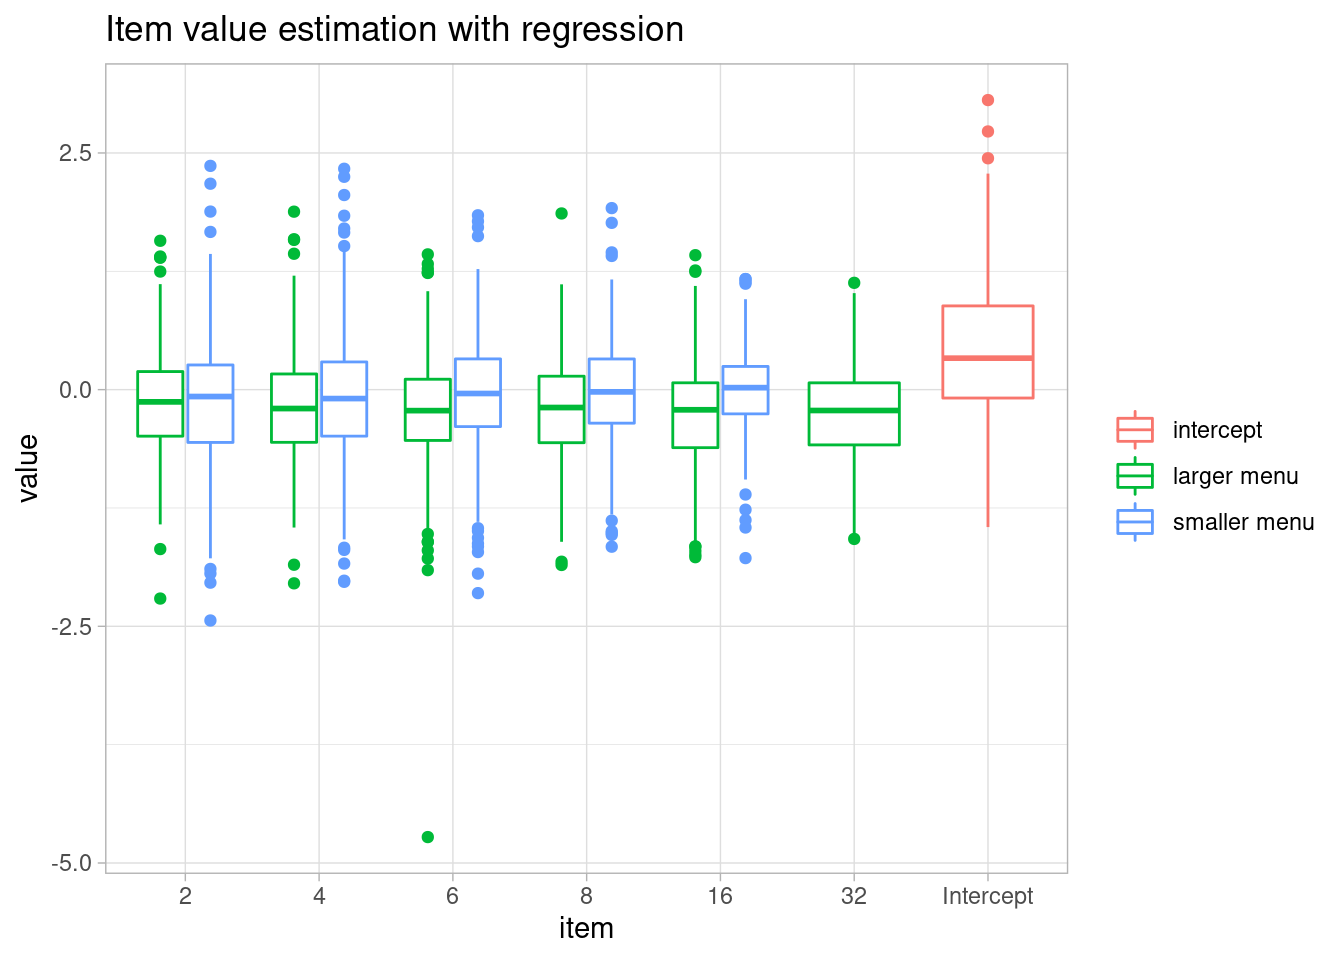
\includegraphics{_main_files/figure-latex/reg-estim-plot3-1.pdf}
\caption{\label{fig:reg-estim-plot3}Distribution of the coefficent by items for all subjects}
\end{figure}

We can see on the graph that the effect in the different variables of the model
are of the same order of magnitude and close to 0.
The estimated values are close to the one estimated for the economic models
especially by comparing the indicator variables for the largest menu with the
preferences for singletons and the one for the smallest menu with the estimates
of the preferences for the temptation. However, it would be premature to
interpret the coefficients of the regression as individual preferences for the
different items.
Indeed our model does not take into account the interaction between the
different variables which could be captured in the estimates of the different
coefficients by bias the the interpretation.
We can however eliminate the hypothesis that subjects evaluate a menu according
to the sum of the items that compose it.
Indeed in this situation there would be no interaction between the different
elements of a menu and we should observe that all the coefficients for the
largest menu are higher or equal to 0 and all those for the smallest menu are
lower or equal to 0, This is not the case here.

As our objective is to use the regression model as a tool for comparison with
other models, we will not try to interpret its coefficients at the individual
level.
We will simply compare the predictions generated by this model with the
predictions of other models and the responses of the subjects.

Now that we have estimated the different parameters for our 5 models, we can
compare their performances using 3 different metrics:

\begin{enumerate}
\def\labelenumi{\arabic{enumi}.}
\tightlist
\item
  Mean Square Error (MSE), which is the mean square difference between the
  predictions of a model and the observed values.
  This metric is the default metric in many machine learning applications because
  of its mathematical form and because it penalizes models with errors that are
  very far from the observations.
\item
  Pearson correlation coefficient, which is an indicator of linear co-tendency
  between two sets of values.
  As our economic models are estimated from relative utility estimates, we use
  this indicator to test that a model is at least consistent with the data in
  terms of trend even if its predictions are biased.
\item
  Percentage of correct sign estimate: our study concerns preferences between
  menus, so we expect a model to be able to correctly predict whether an
  individual will prefer one menu to another or whether he will be indifferent
  between two menus.
  For each model we compute the number of times it predicts a WTC of the same sign
  as the one observed\footnote{Note that the possible observations are +,- or = so it is not an exercise
    of binary prediction or we can improve the predictions of a model by taking the
    opposite of these predictions.}.
\end{enumerate}

In the table \ref{tab:models-table3}, we present the results of the five models according to
the three metrics, calculated on all the comparisons.

\begin{table}

\caption{\label{tab:models-table3}Performance of the models, all comparisons}
\centering
\begin{tabular}[t]{l|r|r|r}
\hline
model & MSE & correlation & correct sign\\
\hline
Linear model & 0.31 & 0.59 & 0.73\\
\hline
G-P temptation & 0.32 & 0.45 & 0.54\\
\hline
Constant response & 0.33 & 0.38 & 0.59\\
\hline
Expected utility & 0.36 & 0.37 & 0.47\\
\hline
Cumulative temptation & 0.46 & 0.33 & 0.56\\
\hline
\end{tabular}
\end{table}

We see that the model that performs best by all metrics is the linear regression
model.
The constant response model is second in terms of percentage of correct sign and
MSE, which tells us that the economic models are globally poor descriptors of
the subjects' behavior.
Among the economic models, we see that the best performing model is the G-P
model.
It is only beaten by the cumulative temptation model for the percentage of
correct sign predicted.
However, the latter model performs very poorly in terms of MSE and correlation.
Finally, if we compare the G-P model with the expected utility model, we see
that taking into account the temptation effect represents a marginal improvement
in descriptive power.
But insofar as these two models perform less well than the constant response
model, it seems unwise to use them.

The table \ref{tab:comp-models-table3} shows the performance of each model according to the type of
comparison.
Before detailing the results, it should be remembered that the different models
were trained using the size 1 menu comparison and the size 2 menu comparison
with the size 1 menus.
These two categories represents 62.86\% of the observations.

\begin{table}

\caption{\label{tab:comp-models-table3}Performance of models by comparaison type}
\centering
\begin{tabular}[t]{l|r|r|r}
\hline
model & 1 vs 1 & 2 vs 1 & other\\
\hline
\multicolumn{4}{l}{\textbf{correlation}}\\
\hline
\hspace{1em}Expected utility & 0.82 & 0.10 & 0.18\\
\hline
\hspace{1em}G-P temptation & 0.82 & 0.36 & 0.18\\
\hline
\hspace{1em}Cumulative temptation & 0.83 & 0.30 & 0.14\\
\hline
\hspace{1em}Linear model & 0.86 & 0.85 & 0.31\\
\hline
\hspace{1em}Constant response & 0.27 & 0.48 & 0.39\\
\hline
\multicolumn{4}{l}{\textbf{MSE}}\\
\hline
\hspace{1em}Expected utility & 0.12 & 0.49 & 0.43\\
\hline
\hspace{1em}G-P temptation & 0.12 & 0.37 & 0.43\\
\hline
\hspace{1em}Cumulative temptation & 0.12 & 0.51 & 0.63\\
\hline
\hspace{1em}Linear model & 0.09 & 0.11 & 0.68\\
\hline
\hspace{1em}Constant response & 0.35 & 0.30 & 0.34\\
\hline
\multicolumn{4}{l}{\textbf{correct sign}}\\
\hline
\hspace{1em}Expected utility & 0.78 & 0.36 & 0.33\\
\hline
\hspace{1em}G-P temptation & 0.78 & 0.51 & 0.37\\
\hline
\hspace{1em}Cumulative temptation & 0.78 & 0.52 & 0.47\\
\hline
\hspace{1em}Linear model & 0.81 & 0.83 & 0.57\\
\hline
\hspace{1em}Constant response & 0.54 & 0.63 & 0.60\\
\hline
\end{tabular}
\end{table}

The first noticeable element in this table is that the different economic models
produce the same results for comparisons between menus of size 1.
The results for this type of comparison are quite good, they are far superior to
those of the constant response model and only slightly inferior to the
regression model.
On the other hand, if we look at the comparisons of size 2 menus against size 1
menus, the performance of the economic models falls below that of the constant
response model.
And this remains true for the other types of comparisons.
The linear regression model is the best model on the training data but it too
performs worse than the constant response model on the new comparison types, it
remains superior to the economic model on these data. This may indicate an
overlearning problem on the training data.

Now if we look at the performance of the economic models we see that the G-P
model performs better than the expected utility model.
It seems that integrating temptation in the evaluation of the comparison between
size 2 and size 1 menus allows to improve the predictions according to our 3
metrics.
But this effect does not seem to have any impact for the other types of
comparisons.
This may indicate that the improvements for the comparison between size 2 and
size 1 menus is due to an overlearning phenomenon.
It may also be a sign that the G-P model does not use the right functional form.
Indeed, alternatives to the G-P model like \citet{noor2015menu} postulate that the
effect of temptation is not linear.
This could be a way to improve the performance of the model for other types of
comparisons but such a model would also be less efficient than a constant
response model for comparisons between menus of sizes 2 and 1, which therefore
does not seem to be a promising direction for improvement.
Finally, the cumulative temptation model is less efficient than the G-P model
except in predicting the sign of the WTCs, but it is still inferior to the
constant response model on this metric too.

We have just seen that economic models are poor descriptors of subjects'
behavior when dealing with menus of more than one option.
In the figure \ref{fig:pred-plot3} we show that these models have in common to
predict that subjects are indifferent between two menus much more frequently
than what we observe.
And that this is also their main difference with the linear regression model
which has better performances.

\begin{figure}
\centering
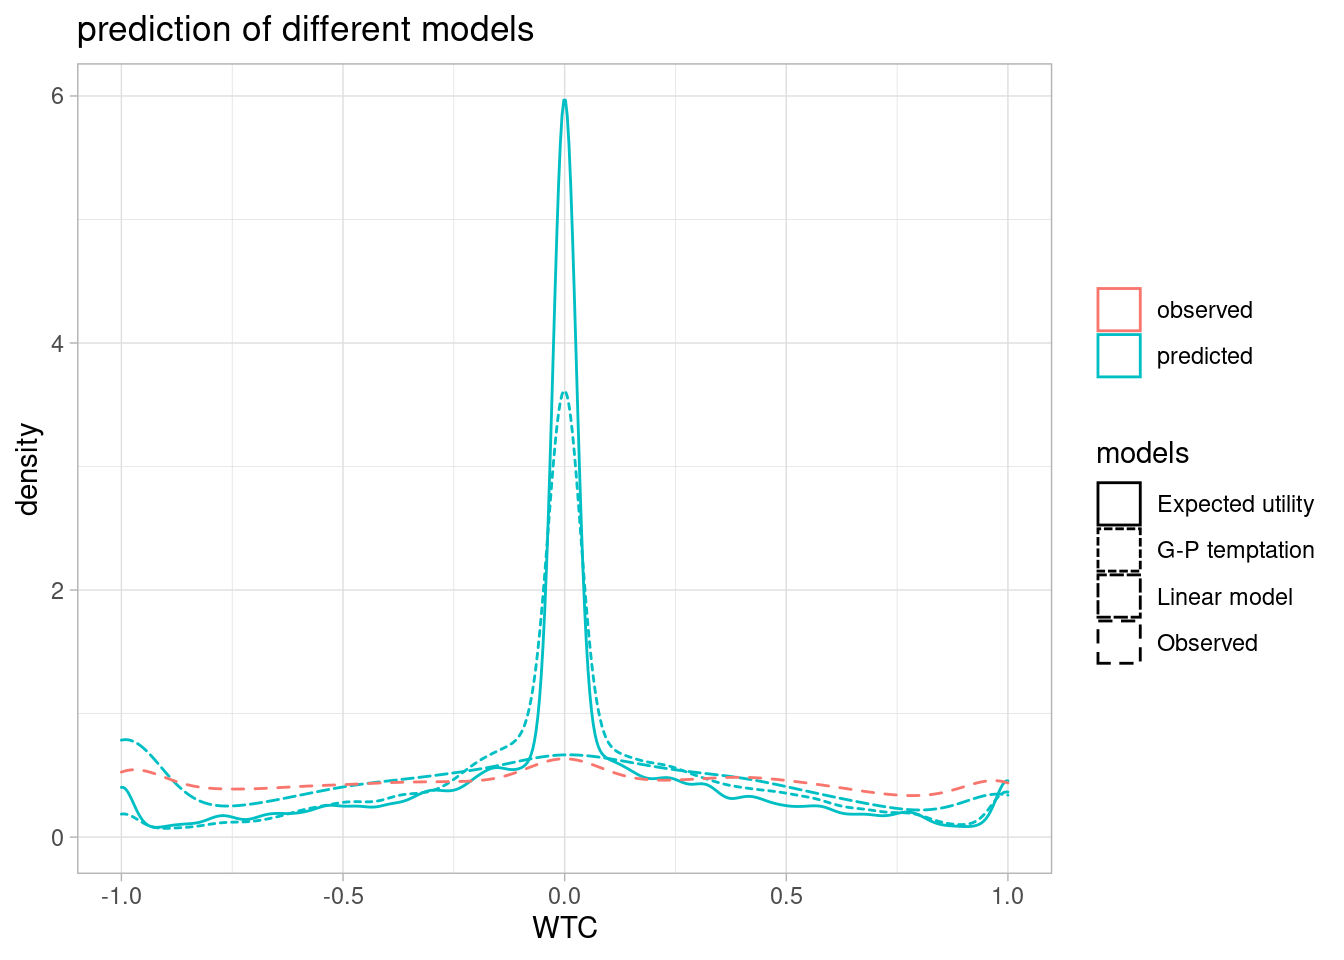
\includegraphics{_main_files/figure-latex/pred-plot3-1.pdf}
\caption{\label{fig:pred-plot3}Distribution of the WTC value predict by models}
\end{figure}

If the economic models often predict the value 0 -- i.e., indifference between
the two compared menus -- this is because they evaluate the
menus according to the preferred item they contain.
In the case of the expected utility model this implies that all menus that share the
same preferred item will have the same estimated value.
In the case of the G-P model this phenomenon is attenuated by the effect of
temptation of another menu item but remains important and the menus that share
their preferred item will have close values.
However, we observe on the comparison of the menus that subjects are rarely
indifferent between two menus.
This seems to contradict the fact that subjects evaluate menus based on a
particular item.

\hypertarget{discu3}{%
\section{Discussion}\label{discu3}}

In this chapter we have proposed an experiment to test the temptation model
proposed in \citet{gul2001temptation}.
In this chapter we have proposed an experiment that compares the descriptive
quality of the model in \citet{gul2001temptation} with other economic and statistical
models.
Our test does not aim at testing the existence of a behavior predicted by the
theory as the rest of the experimental literature on the subject but at testing
the theoretical framework proposed to rationalize this behavior.
Our experiment thus allows us to highlight that the theoretical approach
proposed by G-P does not adequately account for the observed behavior of the
subjects.
We show in effect that a dummy constant response model produces predictions as
close to the observations as G-P's model in terms of precision, tendency and
preference between menus.

Our experiment globally questions the menu choice approach proposed by
\citet{kreps1979representation} and followed by G-P and the temptation models presented
in the review of \citet{lipman2013temptation}.
These models, although an improvement over the expected utility model, are poor
descriptors of our observations.
Their specific item comparison-based approaches underestimate the
difference between two menus reported by our subjects, notably by predicting
that subjects will be indifferent between options over which subjects dare not indifferent.

In this respect, machine learning methods such as simple linear regressions -- that take into account all elements of a menu and not just some preferred ones -- are at least
better descriptors on our data than economic models.
We show in effect that a simple model trained at the individual level offers
better predictions in terms of trend predictions and preferences between menus
than the economic models and the constant response model.

Nevertheless, it should be noted that our analysis, like the menu choice
framework, is based on expected utility theory.
And although we used the most robust estimation methods possible, it is possible
that our results are biased by a discrepancy between the observed behavior of
the subjects and that predicted by the expected utility theory.
Part of this issue will be studied in the next chapter.

We believe that in order to propose models with better descriptive power it
would be useful to have more information on the structure of individual errors.
This would allow us to improve the descriptive performance of risk preference
models as well as models derived from them such as the Gul-Pesendorfer model.

\hypertarget{multi-choice}{%
\chapter{Repeated Choice}\label{multi-choice}}

\hypertarget{intro4}{%
\section{Introduction}\label{intro4}}

In this article we are interested in the following question: When an
individual is confronted several times with the same situation, does he
always make the same choice? This question has few concrete
implications. It is indeed unlikely that an individual is to make two
identical decisions in the same context. But this question seems
important from a theoretical point of view. First, for modeling, the
answer to this question is intimately linked to the choice of
static versus dynamic, deterministic versus stochastic models.
Secondly, for the analysis of results, especially in experimental
economics. Insofar as we consider that individuals always act in the
same way in the same situation, it is only necessary to have one
observation per situation. But if the behavior varies in the same
situation it may be necessary to have multiple observations.

In order to answer this question, we conducted an experiment. We
limited ourselves to a situation where the subjects had to choose
between different lotteries. We chose the risk preference framework for
multiple reasons. First of all, to our knowledge, the question of the
stability of preferences has not been treated in this framework, and
this is a central domain in economics. Moreover, in this field, we have
a theory that has already been widely tested on other themes and whose
extension has difficulty in responding to the contradictions highlighted
by, among others, \citet{friedman2014risky}. These models are for the most part
developments of the von-Neumann and Morgenstern model of expected
utility which is a static and deterministic model. Even the stochastic
models, of which the best known is that of \citet{luce2012individual}, are
built around the existence of a central value for the risk preference
parameters. It seems important to us to question the static nature of
the models used. Finally, from a practical point of view, as the
question of risk preferences has already been treated in experimental
economics, we have tools to measure the parameters of risk behavior. In
our experiment, we will use a variant of the method used in
\citet{lejuez2002evaluation} and \citet{crosetto2013bomb} to elicit the risk
preferences of our subjects. We also have results on similar questions
in the context of risk preferences. For example, \citet{hey1994investigating}
conducted an experiment to test different developments of the expected
utility model. Even if the situations in the experiment were not the
same, this experiment shows the ability of different models to explain
individual decisions. Following the same idea, \citet{wilcox2007predicting}
uses simulations and \citet{hey1994investigating} data to estimate the
predictive power of the models on a new set of situations. Finally, the
\citet{ert2017revisiting}\footnote{We would like to thank Ernan Haruvy for sharing data with us. This allowed us to test our analysis on existing (albeit different) data prior to conducting our experiment.} experiment, which is interested in the learning
of subjects, provides them with feedback and thus modifies the situation
between the different elicitation of preferences, but also studies the
variation of preferences for risk between close situations.

Our experiment was conducted online at the end of May 2021.
The recruitment was done via Amazon Mechanical Turk and we collected data on
300 subjects as planned in our pre-registration\footnote{Pre-registered hypothesis are available with asPredicted code
  \href{https://aspredicted.org/zx667.pdf}{zx667}}.
The experiment itself was done on a dedicated application developed with the
Shiny framework of the R language.
It is built on an extremely simple experimental design. After making sure
that our subjects understood how the risk elicitation task works, we
measured their risk preferences 100 times.
The measurements were taken one after the other without any feedback, the
payoffs and resolution of uncertainty being calculated only at the end of the
experiment.

As the measurements are made in similar situations to each other, we
expect that the 100 measurements will be identical for each subject.
However, we observe that this is only the case for
6.67\% . We show that only for
47.67\% the answers are
normally distributed and that for at least
20.67\% , the data does
not seem to admit a unique central value. Moreover, we show that
measures of risk preferences can lead to the wrong conclusion that a
treatment has an effect.
And that models built on a risk aversion
parameter are of poor quality both in describing the data and in
predicting the future behavior of subjects even in the simplest
situation.
But it seems possible to significantly improve the quality of
predictions by using models that take into account the past behavior of
the subjects.

Our experiment shows that it should not be taken for granted that when
confronted with the same situation several times an individual will
always respond in the same way.
Responses can vary significantly not only between but also within subjects.
Within-subjects variations can be so extreme
that the behavior of a subject cannot be satisfactorily summarized
by a central value.
This implies that we must pay particular attention
to the conclusion that we draw from a difference between two measures,
but also to the behavioral conclusion that we can deduce from a risk
aversion parameter.
Finally, these results must be put into perspective
by the fact that our experiment has few equivalents and that,
consequently, the results we have obtained are uncertain and must be
supported and corrected by other studies.

\hypertarget{mm4}{%
\section{Experimental design}\label{mm4}}

Our experimental design allows us to measure 100 times the risk
preferences of each subject. Each of these measurements is performed
under conditions as close to each other as possible. Each of the
measures is performed using an elicitation mechanism regularly used for
similar purposes in economics and psychology. Each of the elicitations
is incentivized by an amount that even if relatively small in absolute
value is much higher than the average remuneration used in experimental
economics on the target population. Moreover once the amount is put in
relation to the effort and duration of the task, the corresponding
remuneration is similar or even higher than the remuneration of subjects
in laboratories. Our protocol also includes a learning period with
feedback in addition to the traditional control questions in order to
ensure that the subjects have fully understood how the elicitation
procedure works and its impact on their compensation.

We believe that our experimental design allows us to satisfactorily
study how individuals behave in the face of risk on a repeated basis. We
have a large number of observations per subject which allows us to
perform robust statistical analyses at the individual level. And the
observations are comparable at the individual level because we made sure
that the conditions are as close as possible in terms of incentive,
information, form and time.

Our experiment took place from May 25\textsuperscript{th} to May 27\textsuperscript{th}, 2021.
It involved 300 subjects\footnote{317 subjects finished the experiment but only those
  having entered a valid payment and control code at end of experiment were taken into
  account in the analysis.}.
The recruitment was done using Amazon Mechanical Turk and no
constraint of competence or localization was applied.
The subjects were
paid a fixed amount of 0.5\$ plus a variable amount depending on the
lotteries they chose.
In order to ensure the quality of the answers provided
and rule out automatic replies by bots,
we controlled for a number of parameters on the answers provided by
our subjects:

\begin{enumerate}
\def\labelenumi{\arabic{enumi}.}
\tightlist
\item
  A response time for the experiment of less than 10 minutes.
\item
  A number of trials higher than 3 for the control questions.
\item
  A number of changes in the answer before validation less than 112
  (the minimum possible is 110) or more than 200.
\item
  A small variation in response time to the lottery (a standard
  deviation of response time of less than 1 second).
\item
  A small variation in response time between responses (a standard
  deviation of time less than 2 seconds).
\end{enumerate}

None of these criteria is in itself a sign of poor response quality, but
the combination of several of them could be problematic.
Fortunately, only 23 subjects accumulated 2 and only 2 accumulated 3 (and no
subject was flagged for 4 or more criteria).
This leads us to believe that the answers provided by the
subjects can be considered of good quality and not polluted by
automatic answer programs.

The course of the experiment for the subjects was as follows:

\begin{enumerate}
\def\labelenumi{\arabic{enumi}.}
\tightlist
\item
  The subjects select the task on Amazon Mechanical Turk, they are
  informed of the approximate duration as well as the amount of the
  fixed payment and the nature of the task. They are presented with a
  link to the experiment.
\item
  When they arrive at the experiment website, they are presented with a login
  screen that asks them to choose a username and password (or to
  provide their own if they have experienced a logout problem). If the
  identifiers are valid they are secretly and randomly assigned to one of the 9
  treatments.
\item
  The instructions of the experiment are presented to them. The instructions
  explain the process of the task as well as how they will be rewarded
  according to the lotteries they have chosen.
\item
  The subjects are then asked to answer 4 simple control questions.
  They have as many tries as they want to find the right answers, but
  they have to succeed in order to continue.
\item
  The subjects of the treatments concerned must then answer a
  questionnaire on risk behavior.
\item
  Subjects are then asked to select 10 lotteries and are shown the
  bonus they would have obtained based on their choices, but they are
  warned that these lotteries will not affect their bonuses. This step
  serves as a learning phase so that the subjects can take the
  mechanism in hand by themselves.
\item
  Subjects select the 100 lotteries that will be used to calculate
  their bonus. This phase represents the main body of the experiment.
\item
  The subjects of the concerned treatments have to answer a short
  questionnaire about their preference for the risks similar to the
  one at the beginning of the experiment.
\item
  The lotteries that will be taken into account for the subjects'
  bonus are drawn and uncertainty resolved in order to calculate the bonus of each subject.
  The results are presented in a table with a summary of the gains as
  well as the code to be filled in on Amazon Mechanical Turk so that
  the subject can receive the bonus. Only the subjects correctly filling the code to AMT are paid and kept for the analysis.
\end{enumerate}

Our experiment includes 9 treatments, over two independent dimensions, each with
3 modalities.
The first dimension concerns the risk behavior questionnaire, that can be run at
the beginning, at the end of the experiment or both.
The second dimension concerns the lotteries proposed to the subjects.
The 3 modalities are the following:

\begin{enumerate}
\def\labelenumi{\arabic{enumi}.}
\tightlist
\item
  Each lottery is presented on a separate screen and each of the 100
  lotteries is payoff-relevant.
  Each experimental currency unit is worth 0.005\$.
\item
  The lotteries are presented 10 per screen and one lottery per screen
  is randomly drawn to be payoff-relevant. Each experimental currency unit
  is worth \$0.05.
\item
  The 100 lotteries are presented all on one screen and a single lottery
  is randomly drawn to be payoff-relevant. Each experimental currency unit
  is worth \$0.5.
\end{enumerate}

In each of the treatments the maximum expected payoff is \$8.
The different treatments should not impact the behavior of the subjects, the
situations being theoretically similar.
Having different payment modality is a robust test against the bipolar
behaviorist bias pointed out by \citet{harrison2014experimental}.
However, we cannot use any of our processing to perform robustness tests.
Our analysis of the data revealed a ghost treatment effect (detailed in the
following analysis) which may make treatments appear statistically different
without reason.
We therefore chose to conduct the analysis by pooling the treatments.

Incentives may seem too small, but this is not the case.
The maximum average gain for our experiment is \$8.5 which
makes it an extremely well-paid task given that the average time to
complete it is 42
minutes.
This amount is also extremely dependent on the subject's choices.
It can indeed vary from 0.5\$ to 8.5\$ depending on the choice,
and even in treatments where the value of a unit is 0.005\$ the amount
expected from a lottery can vary from 0\$ to 0.08\$ which may seem low
but should be put in comparison with the time needed to make this
decision (in the order of a second) and the amount usually paid for
tasks on Amazon Mechanical Turk (e.g. \citet{sjaastad2021ulyssean} pays
subjects 0.01\$ to correctly count the number of colored cells in a 150
cell matrix in 50 seconds). This leads us to believe that the collected
responses reflect, a decision similar to the
one usually observed in experimental economics when eliciting
responses from subjects in a brick-and-mortar laboratory.

The objective of our experimental design is to have subjects make the
same choice multiple times (or at least choices that are as close as
possible) and to incentivize them, within the framework of utility
theory, to make the same decision each time. We have therefore chosen to
repeat the same risk elicitation task 100 times in a row. The
repetitions are done one after the other without any feedback until the
end of the experiment. The different elicitations are performed in a
short time (less than 2 hours for the slowest).
The different choices do
not or can not differ between them in terms of information, time or gain
already acquired. The main difference is that as the experiment
progresses, the number of decisions made by a subject increases, but
this factor does not influence decision making in the expected utility
model (and in many other models in decision theory).

To ensure that subjects are encouraged to make the same decision in each
of their choices, we chose to use an elicitation method inspired by the Balloon
Analaog Risk Task (BART, \citet{lejuez2002evaluation}) and the Bomb Risk Elicitation
Task (BRET \citet{crosetto2013bomb}).

Our task is the same as BART but without the ball.
Removing the balloon is a way to avoid the subject being distracted by the
balloon animations or being biased by his experience with real ball as
highlighted in \citet{steiner2021representative} and \citet{de2020burst}.
In our task subjects have to choose a value \emph{n} between 0 and 64.
This value corresponds to a lottery which allows them to win \(n\) units (whose
value depends on the treatment as explained later) with a probability of
\(\frac{64 - n}{64}\) and 0 otherwise.
By considering subjects whose utility function is of the CRRA
type and using the form used by \citet{wakker2008explaining}:
\[
u(x) = 
\begin{cases} 
  x^r & \text{if } r>0\\
  -x^r & \text{if } r<0\\
  ln(x) & \text{if } r=0
\end{cases}
\]
We can show that this task allows to elicit the preferences of
individuals with a risk aversion parameter between 0.016 and 64. And
that for a value r between these 2 values :
\[
n^* = \frac{64r}{1 + r}
\]
With \(n^*\) the value that maximizes the utility function \(u(\cdot)\). We can
also associate to each possible value of \(n\) the parameter \(r\) for which
the utility function would be maximized (except for the values 0 and 64
which are choices strictly dominated by all others):
\[
r = \frac{n}{64 - n}
\]
For each iteration of the task performed by a subject, we can
therefore easily associate a risk aversion parameter.

\hypertarget{result4}{%
\section{Results}\label{result4}}

Our analysis will be composed of 3 parts.
In the first part we will describe the individual choices in terms of variance
and associated distributions.
In doing so we will show that individual behavior is highly variable and that
they are not normally distributed as is often assumed in economic data analysis.
In the second part we will show the consequences of these specificities
and their impact on the statistical methods used to test hypotheses and
the reliability of the results. Finally, we will briefly look at a
potential way to improve the methods usually used to estimate risk
aversion.

Using the elicited values we will estimate different models.
We will then compare these models according to their Mean Square Error (MSE) on
subsets of our data of different sizes.
In all situations we adopt the standard practice in machine learning of training
the models on sets distinct from the test set on which we measure the MSE.
The models we use are the following:

\begin{enumerate}
\def\labelenumi{\arabic{enumi}.}
\tightlist
\item
  \textbf{dummy}: This model simply predicts for each subject and each
  period 32.
  This value is the central value among those available.
  This model does not learn anything about the behavior of the
  subjects and is only used as a reference to judge the performance of
  the other models.
  The models performing less well than this model are probably not relevant.
\item
  \textbf{mean, median, mode}: These models predict for each subject the simple
  mean/median/mode of the values observed during the training periods.
\item
  \textbf{r\_irr}: This metric is proposed to have a metric that internalizes
  individual errors.
  We therefore use this index \emph{r of irrationality} which for a set of choices of a
  subject indicates the value r which minimizes the irrationality in terms of
  certain equivalent.
  This model predicts the value corresponding to the specific risk
  aversion parameter \(r\) of a CRRA utility function
  that minimizes for each subject its irrationality index over
  the learning period.
  We define irattionality index as the sum of the
  difference between the certainty equivalent chosen by the subject
  and the certainty equivalent of the optimal choice for a given
  utility function.
  \[
  d_{irr} = \sum_{i =1}^{i = N}c(n^*, u)-c(n_i, u) 
  \]
  with \(c(n, u)\) the certainty equivalent of the choose \(n\) for
  an individual with an utility function \(u\), and \(n^*\) the choice that
  maximize the utility function \(u\).
  From this metric we estimate utility function for subject by minimising
  \(d_{irr}\).
  This model has the advantage of being able to be calculated for different sets
  of choices and to take into account the strictly dominated choices made by a subject.
\item
  \textbf{r\_local}: This model predicts for each subject the value
  corresponding to the average of the r-values calculated for each
  training period. This model has the advantage that it can be
  computed for different sets of choices like the previous one.
\end{enumerate}

The first notable feature of our results is the significant heterogeneity in
individual behavior. Indeed, the subjects have in the experiment
extremely different attitudes both in terms of average values chosen and
variance around this average. But even for the individuals closest to each other
in terms of mean and variance there can be significant differences in behavior
both in the frequency of variations and in their amplitudes.
Figure \ref{fig:spag-plot4} gives a visual glimpse of the behavioral
heterogeneity.
Each line corresponds to the choices of an individual and the individuals are
divided by increasing average choice over the rows and by increasing variation
over the columns.
Each cell of the graph contains 12 individuals.

\begin{figure}
\centering
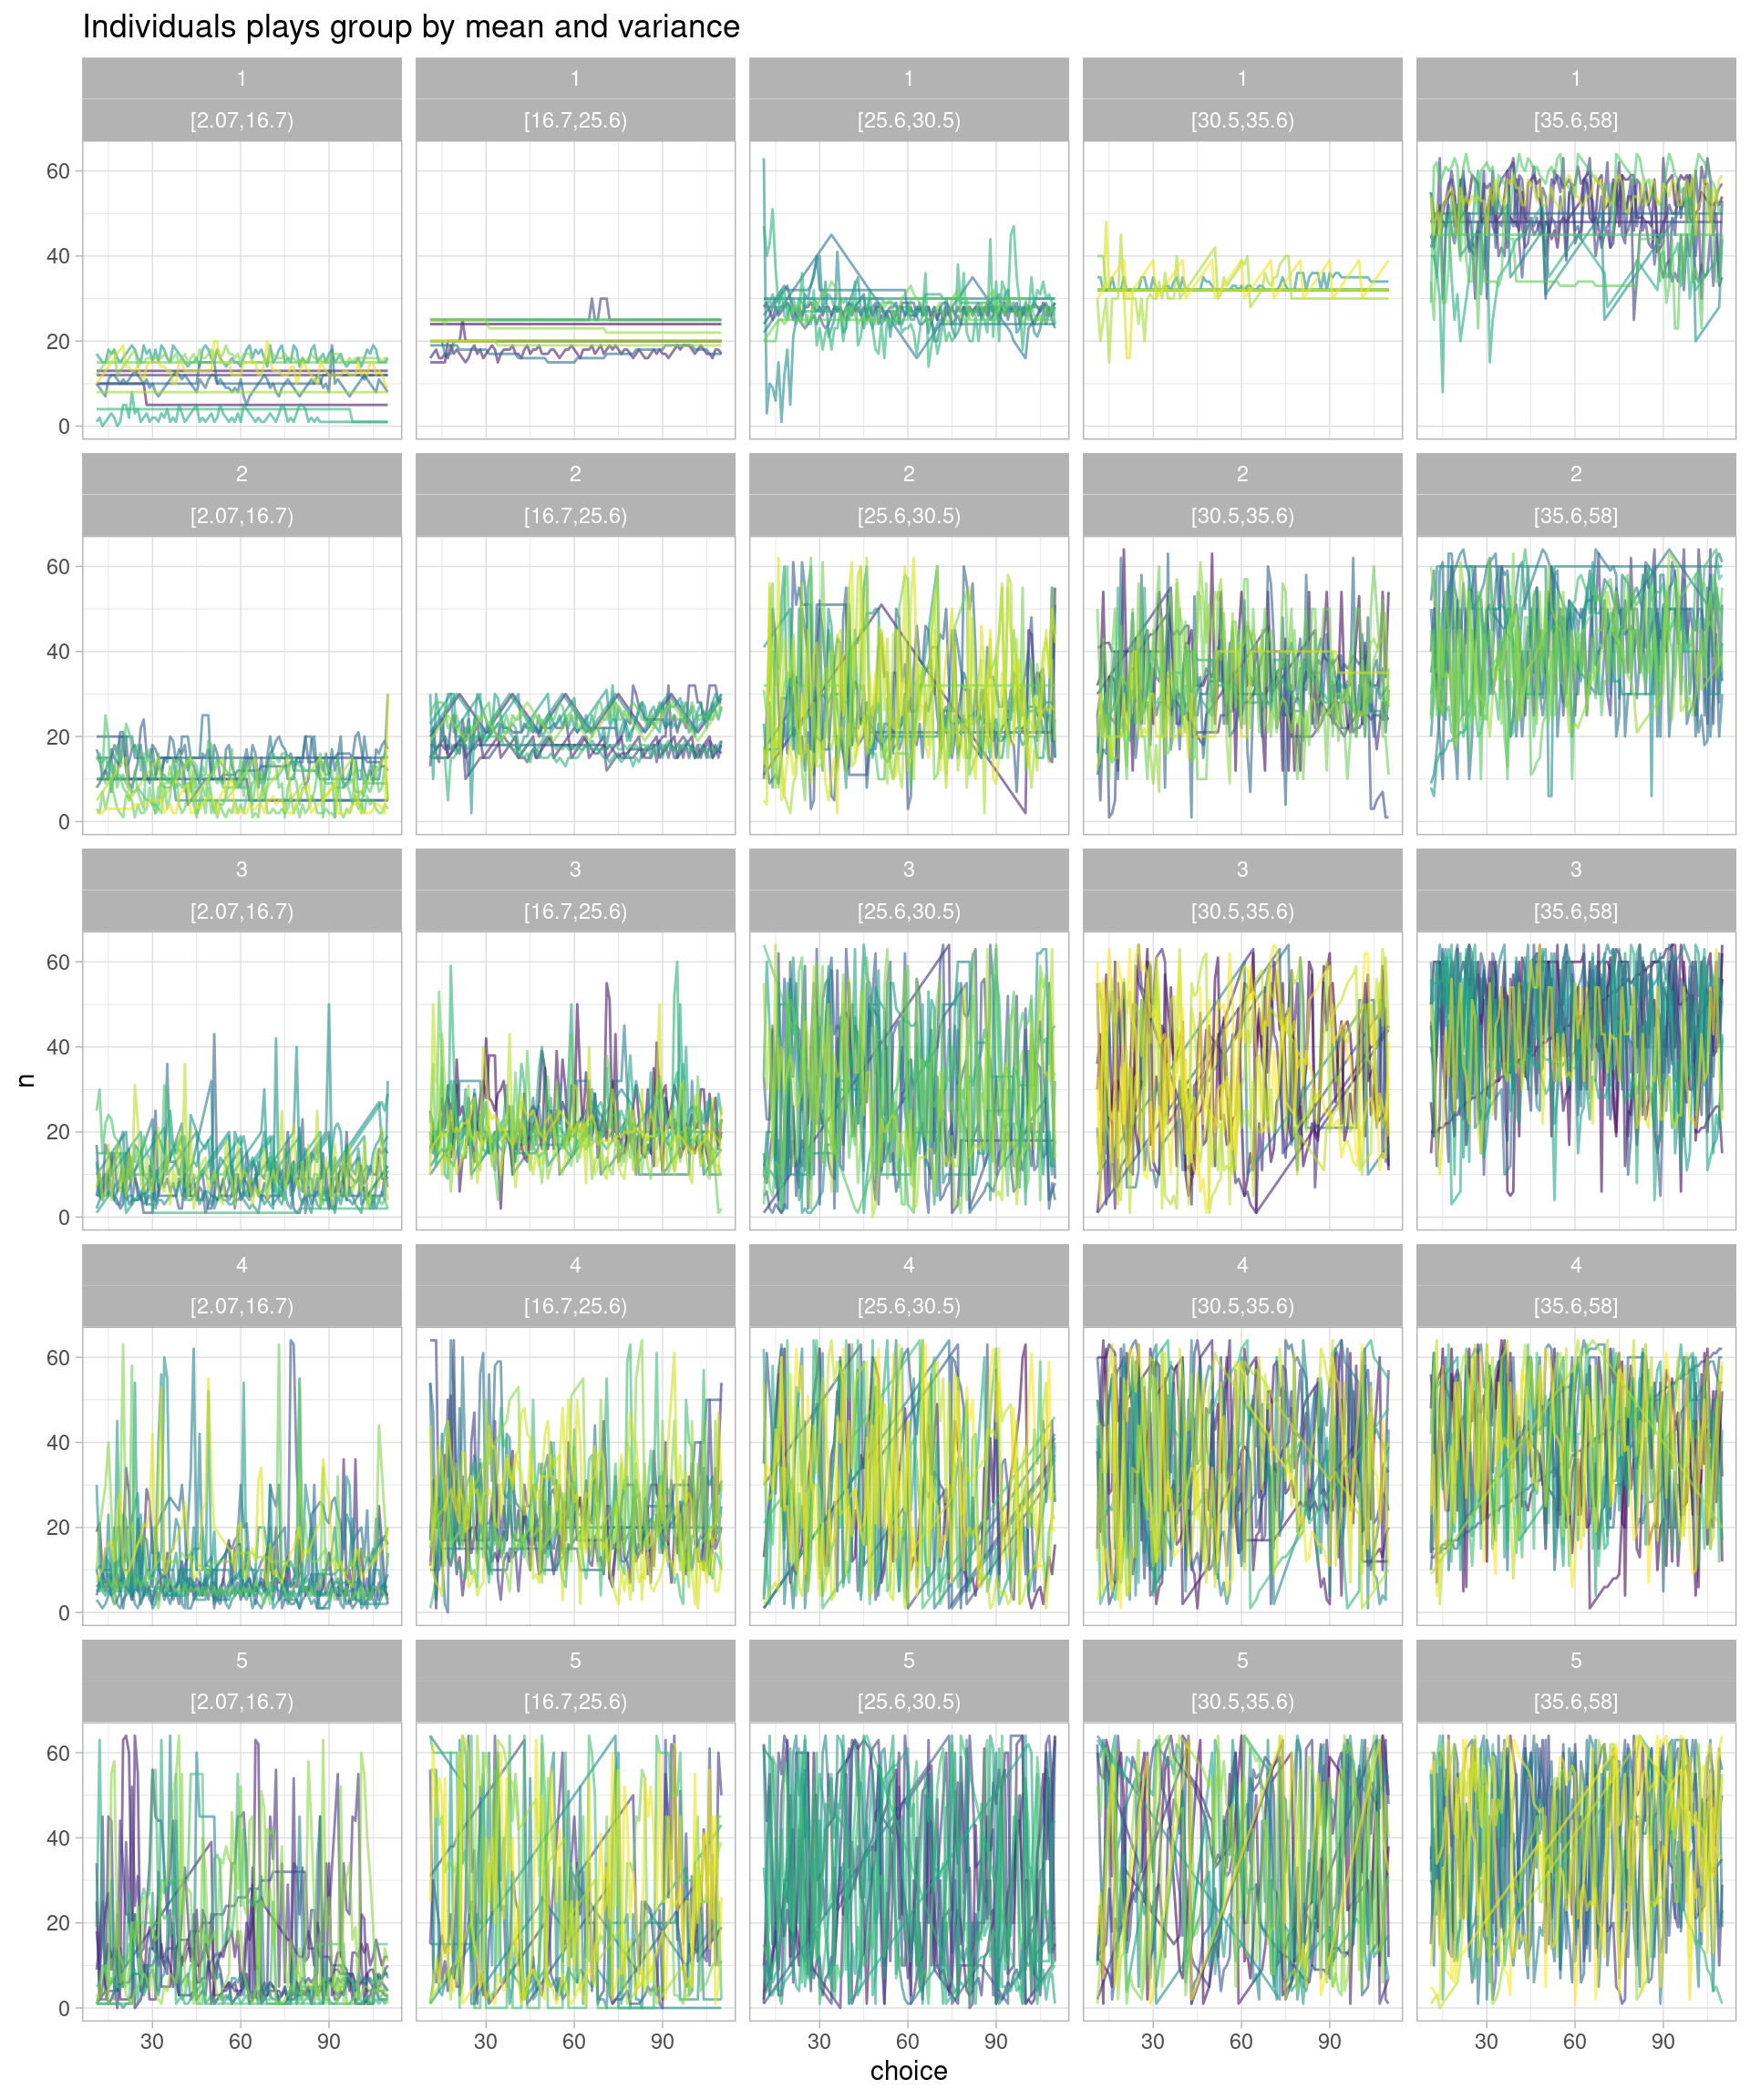
\includegraphics{_main_files/figure-latex/spag-plot4-1.pdf}
\caption{\label{fig:spag-plot4}All choice. Each line show the 100 choices of a subject}
\end{figure}

This large variation in individual behavior is less evident in the
statistics.
In the table \ref{tab:sum-stat-table4} we have reported the
quantiles of the mean and standard deviation per subject.
In this table we have also indicated the quantiles for the 95\% confidence
interval for the parameter \(r\) per subject under the assumption of normal data,
as well as the part of the observations that should be outside the observed
values (inferior to 0 or superior to 64) under the assumption of a normal
distribution.

\begin{table}

\caption{\label{tab:sum-stat-table4}Statistique of individual choice}
\centering
\begin{tabular}[t]{l|r|r|r|r|r}
\hline
  & quantile 5\% & quantile 25\% & median & quantile 75\% & quantile 95\%\\
\hline
mean & 7.56 & 19.06 & 27.64 & 34.47 & 45.06\\
\hline
sd & 0.00 & 4.35 & 11.43 & 16.50 & 19.10\\
\hline
mean r & 0.19 & 0.61 & 1.66 & 3.97 & 7.47\\
\hline
sd r & 0.00 & 0.16 & 2.94 & 9.71 & 14.71\\
\hline
width of r C.I. & 0.00 & 0.55 & 3.92 & 63.76 & 64.00\\
\hline
\% estim not in [0,64] & 0.00 & 0.04 & 4.19 & 7.73 & 16.54\\
\hline
\end{tabular}
\end{table}

Average results are consistent with
the literature on risk attitudes in the laboratory. The majority of the subjects
are risk averse (average \(n\) lower than 32) and very few subjects have an
average higher than 48 (theoretical equivalent to an \(r\) of 3). On the
other hand, with a median standard deviation of
11.43 the variability of the data is
extremely high. This variability makes us think that the behavior of the
subjects does not come down to a constant choice with a low variability
around this choice. In any case, this variability has a major impact on
the estimates of a risk aversion parameter from these data. Indeed, if we
calculate the confidence interval for the parameter \(r\) per subject from
the average choice and the standard deviation observed under the
assumption of normality of the data, we obtain extremely wide intervals
as shown in the corresponding column of table \footnote{Note that as under the assumption of normality it is possible to
  observe values of n lower than 0 (and higher than 64) the values for
  the parameter r were brought back to 0 (and to 64) for the extreme
  cases and that this reduces the size of the reported confidence
  interval.}.

This high variability also makes the hypothesis that the data is
approximately normally distributed aberrant.
For at least half of the subjects
we would have under the hypothesis of normality more than
4.19\% of the data which would not be
included between 0 and 64\footnote{To claim that our results can be described with a normal distribution
  would be similar to saying that a model that predicts that the height of
  4.19\%\% of humans is less than 0 cm or greater
  than 3m accurately describes reality.}.
To finish with the hypothesis of normality of the individual choices, a
Kolmogorov-Smirnov\footnote{As normality test are sensitive to ties, and our observations are integer
  and this contain ties, we add an uniform noise to observation before running the
  test.} test was carried out by individual on their choice.
For 52.33\% of the subjects
the test rejects the hypothesis of normality of the data at a threshold
alpha of 5\%.
We are therefore confident that a normal approximation is a poor representation
of the behavior of our subjects, especially for some of them.

Can the behavior of individuals be described using a central value?\\
To test this we calculate for
each individual their mean choice 5000 times, drawing 75 out of the 100 choices
and then we test if these different values of the mean are
normally distributed. This method consists in testing the central limit
theorem on the individual bootstrapped mean. We
use 3 different normality tests to ensure the reliability of the
results obtained. The tests used here are the Kolmogorov-Smirnov
(KS), the Shapiro-Wilk (SW) and the Anderson-Darling test (AD).
Each test is based on a different criterion and we expect to have
different but consistent results. In the table \ref{tab:norm-test4}, we report for each
test and their different combination the percentage of subjects for whom
the test is not considered significant at the 5\% alpha level.

\textbackslash begin\{table\}

\textbackslash caption\{\label{tab:norm-test4}Share of subject who choice pass normality test at 5\%\}
\centering

\begin{tabular}[t]{rrrrr}
\toprule
KS & SW & AD & KS \& SW \& AD & KS or SW or AD\\
\midrule
69.67 & 54.33 & 60.67 & 43.33 & 79.33\\
\bottomrule
\end{tabular}

\textbackslash end\{table\}

The normality tests show that for a significant proportion of subjects,
the mean is not normally distributed. The proportion of subjects varies
according to the test, from 30.33\%
for the Kolmogorov-Smirnov test to
45.67\% for the Shapiro-Wilk test.

This difference is explained by the statistics used, the
Kolmogorov-Smirnov test takes into account the maximum deviation between
the empirical distribution and the theoretical distribution while the
Shapiro-Wilk test tests the difference between the ordered values and
the observed values. We can say that the share of the subjects concerned
is between 56.67\% and
20.67\% but it is difficult to
give an exact value.

Beyond the fact that this confirms that individual data are not normally
distributed for a significant number of subjects, it raises an even more
important issue. Indeed, if the mean of the individual data itself is
not normally distributed, this indicates that we are in a situation
where the central limit theorem does not apply. This may have two
causes, first, our sample is too small to allow the mean to converge.
This would be problematic given that the number of data per individual
that we have is much higher than what is usually done in experimental
economics. Moreover, it would suggest that the data are distributed
according to a probability distribution for which it is necessary to
observe a large number of data to obtain a reliable estimate of the
mean, which excludes most of the distributions usually used to model
this type of data. Second, the decision process of the subjects is of a
type that does not admit first and second order moments.
This result shows us that random choice models such as \citet{gul2006random},
\citet{gul2014random} or \citet{cerreia2019deliberately} are not suitable to describe the
choices of our subjects.
These models have in common that even if the choices of the subjects can vary
between 2 iterations they should be distributed around a central value in this
situation.

While the results reported above might seem like technicalities, we will show
that they have implications for the methods used and the results reported in
risk elicitation studies.
The first impact of the way individuals choose is on the statistical methods
used to test hypotheses in experimental economics.
The commonly used approach is to
separate the observations that will be available according to the
application or not of a treatment. We distinguish here three approaches.
The first one, which is called in between, consists in applying the
treatment to a part of the subjects and not applying it to another part,
and in comparing the two groups. The second approach, called within,
consists of applying the treatment to all subjects but on a subset of
the observations collected by subjects, and comparing the results
between the periods when the treatment was applied or not. The last one,
the difference in difference (diffDiff) approach, consists in combining
the two other approaches. The subjects are separated in two groups and
the treatment is applied only to a part of the observations of one
group, which allows to compare the differences of variations between the
two groups for the periods when the treatment is applied or not. The
comparison is then generally made using a test of equality of means
between the groups.

We propose here to study ghost treatment. That is to say that we randomly group
our observations as if our subjects had been subjected
to a treatment when in fact they were not.
To simulate a between-subjects treatment, the same number of subjects
were randomly drawn from each group.
To simulate a within-subjects treatment we draw a
period and we take for each subject the same number of observations
before and after this period.
To simulate a difference-in-difference
treatment we apply the same method used for within-subjects treatments but with
two randomly selected groups as done for between-subjects treatments.
For the first type, we
compare the means of the \(n\) between the 2 groups with the help of a
Student's t test. For the difference in difference simulations we
compare the difference in means between the groups for the differences
between the periods using the same test. For each of the presented
approaches we test the results with a bootstrap method on individuals
and periods.
For each of the parameters we performed 5000 draws.
For each draw we performed a test with a type I risk threshold of 5\%.
In the figure \ref{fig:gt-plot4} we present the share of the draws for which the
differences in behavior were judged as statistically significant (note
that the ordinate axis is presented as a \% of the maximum choice made by
the subjects which is 100 in between and 50 for the other methods).

\begin{figure}
\centering
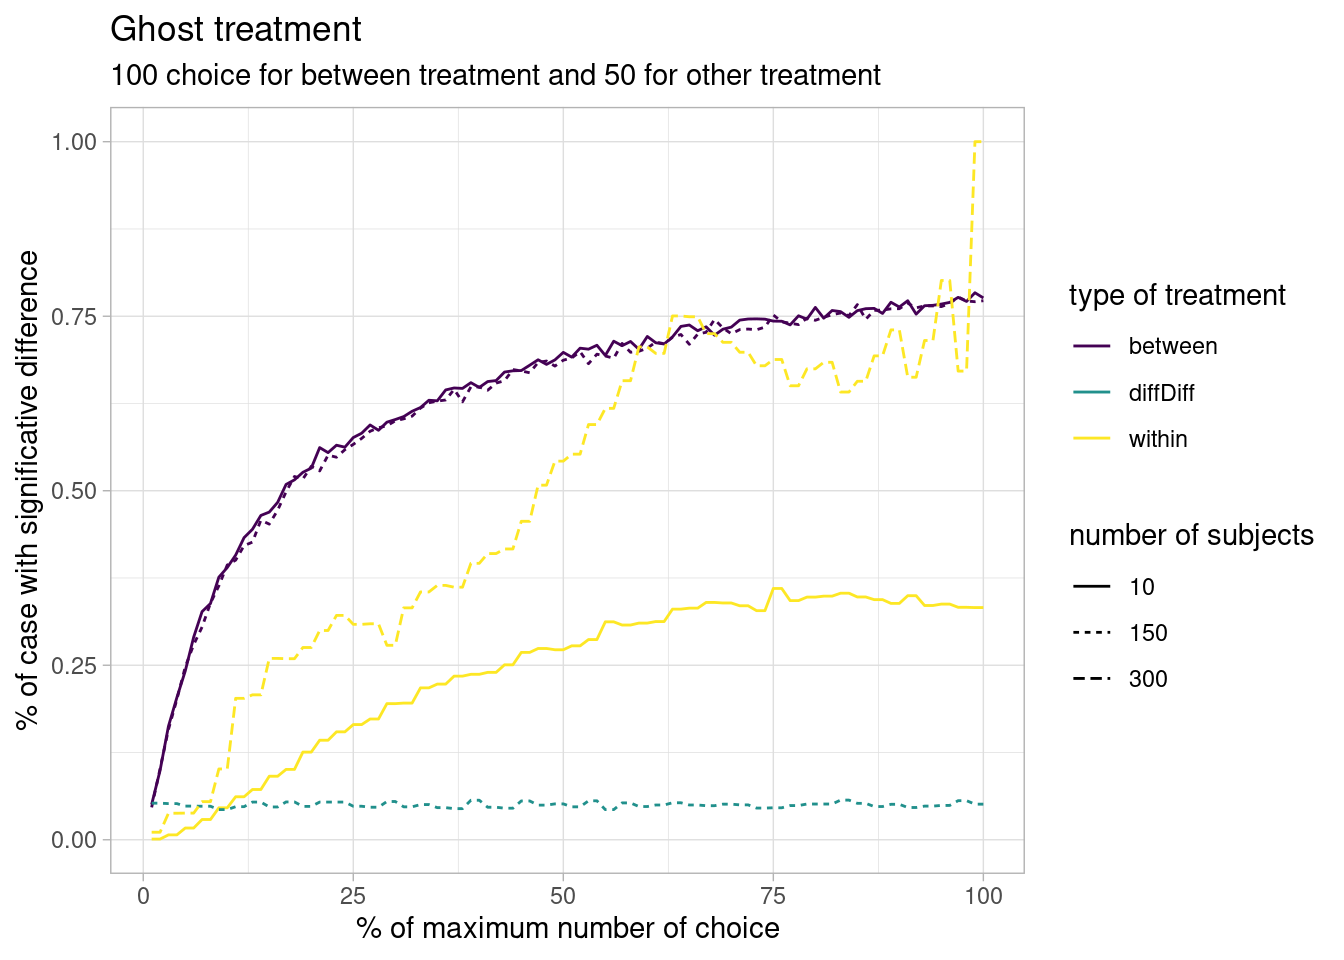
\includegraphics{_main_files/figure-latex/gt-plot4-1.pdf}
\caption{\label{fig:gt-plot4}Bootstrap t.test at 5\% levels for different design}
\end{figure}

Since the groups are randomized, it is expected that the rate of
significant cases will be equal to the type I error, that is 5\%.
Especially in within as no or little individual variation is assume in the
experimental litterature.
But we notice that only the difference-in-difference method gives the expected
result.
The two other methods present a rate of significant cases much
higher than what is expected, higher than 75\% when we use all the
observations we have.
This rate of significant cases seems to be little
affected by the number of subjects, in the case of the between-subjects method
the number of subjects does not even seem to have any impact On the
other hand, this rate seems to increase with the number of observations
per subject.

This situation is particularly problematic if we wish to
test a hypothesis on individual behavior, because taking too few
observations leads to low power and increasing the number of
observations without using adequate methods leads to a high risk of
wrongly detecting an effect.

Another element in data is the low correlation of risk elicitation task with
itself.
We tested the correlation of the observations between different periods.
The periods were selected using three different methods:

\begin{enumerate}
\def\labelenumi{\arabic{enumi}.}
\tightlist
\item
  \emph{random}: the periods were randomly drawn without replacement to form
  two groups of equal size.
\item
  \emph{ordered}: the periods were randomly drawn without replacement
  before and after a value randomly drawn to form 2 groups of equal
  size.
\item
  \emph{consecutive}: the same number of consecutive periods were drawn before and
  after a randomly drawn value. This method is the closest to an
  experiment consisting in testing the correlation of the elicitation
  task with itself.
\end{enumerate}

For each of these methods we used a bootstrap method on the number of
periods and we made for each value 5000 draws. The figure \ref{fig:corr-plot4}
shows the evolution of the average correlation by method as a function of the
number of periods.

\begin{figure}
\centering
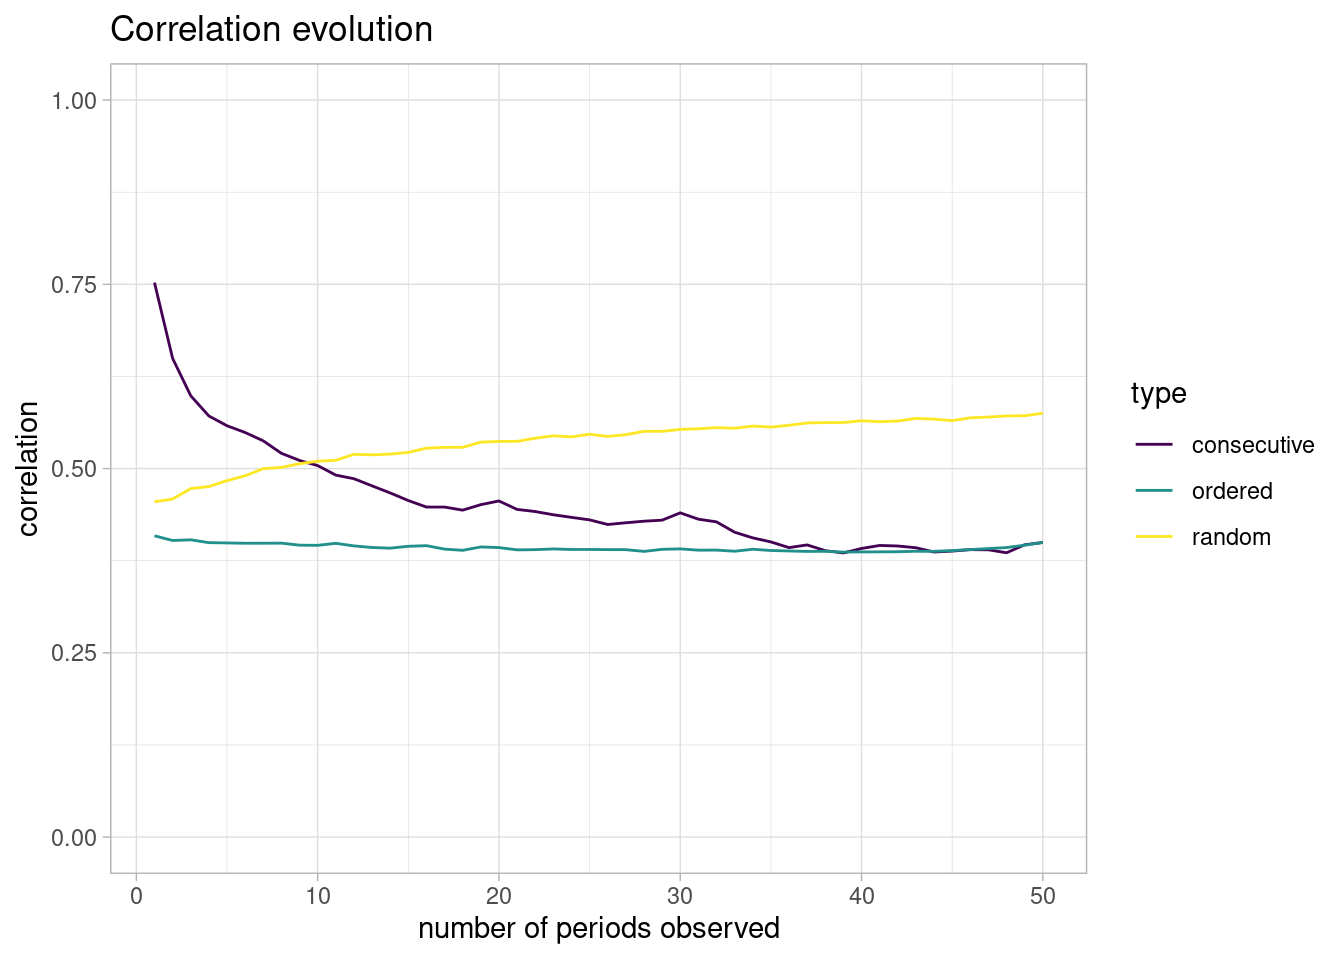
\includegraphics{_main_files/figure-latex/corr-plot4-1.pdf}
\caption{\label{fig:corr-plot4}Pearson corelation between subject choice.}
\end{figure}

As in theory we measure the correlation between independent and
identically distributed observations, we expect the measured correlation
to be close to 1, only subject to random sampling variations and
identical for the 3 methods.
But we observe that the measured
correlation varies between the three methods. Except for the ordered
method whose result seems to be independent of the number of periods,
the two other methods show a clear trend with the increase of the number
of periods considered. The average correlation measured by the consecutive method
is decreasing with the number of periods, while it is increasing for the
random method. Moreover, the average correlation remains relatively low
compared to what is theoretically expected. Indeed, all methods and
number of observations taken together, it is between
{[}0.39, 0.75{]}. And
for the consecutive method with 50 observations per subject it is only
0.4.
The observed correlation is therefore much lower than 1.
The risk elicitation measure is therefore less correlated with itself than one
would expect.
This must be taken into account in studies where different risk measurement
methods are compared as in \citet{crosetto2016theoretical}.
In this kind of exercise the correlation observed between two methods can be low
compared to the theoretical value of 1 but be quite close to the correlation
that a method has with itself.
Beyond these practical considerations, this correlation of
0.4
tells us that our method of eliciting risk preferences is not reliable to
indicate that an individual is more risk averse than another;
indeed the ranking between individuals is likely to be different between 2
measures.

An issue related to the question of correlation is the question of the
predictability of future behavior.
This question has to our knowledge been little studied, and never on the same
set of choices as the one used for the learning of behaviors.
We will therefore compare different estimators according to the quality of their
prediction on a set of observations different from the training set.
This is cross validation, a commonly used method in machine learning.
It allows to compare models while avoiding overfitting problems.
In the figure \ref{fig:plt-error-model4} we show the
results of different models according to the number of periods devoted
to learning (the number of test periods and 100 minus the number of
observations devoted to learning) in terms of mean square error.

\begin{figure}
\centering
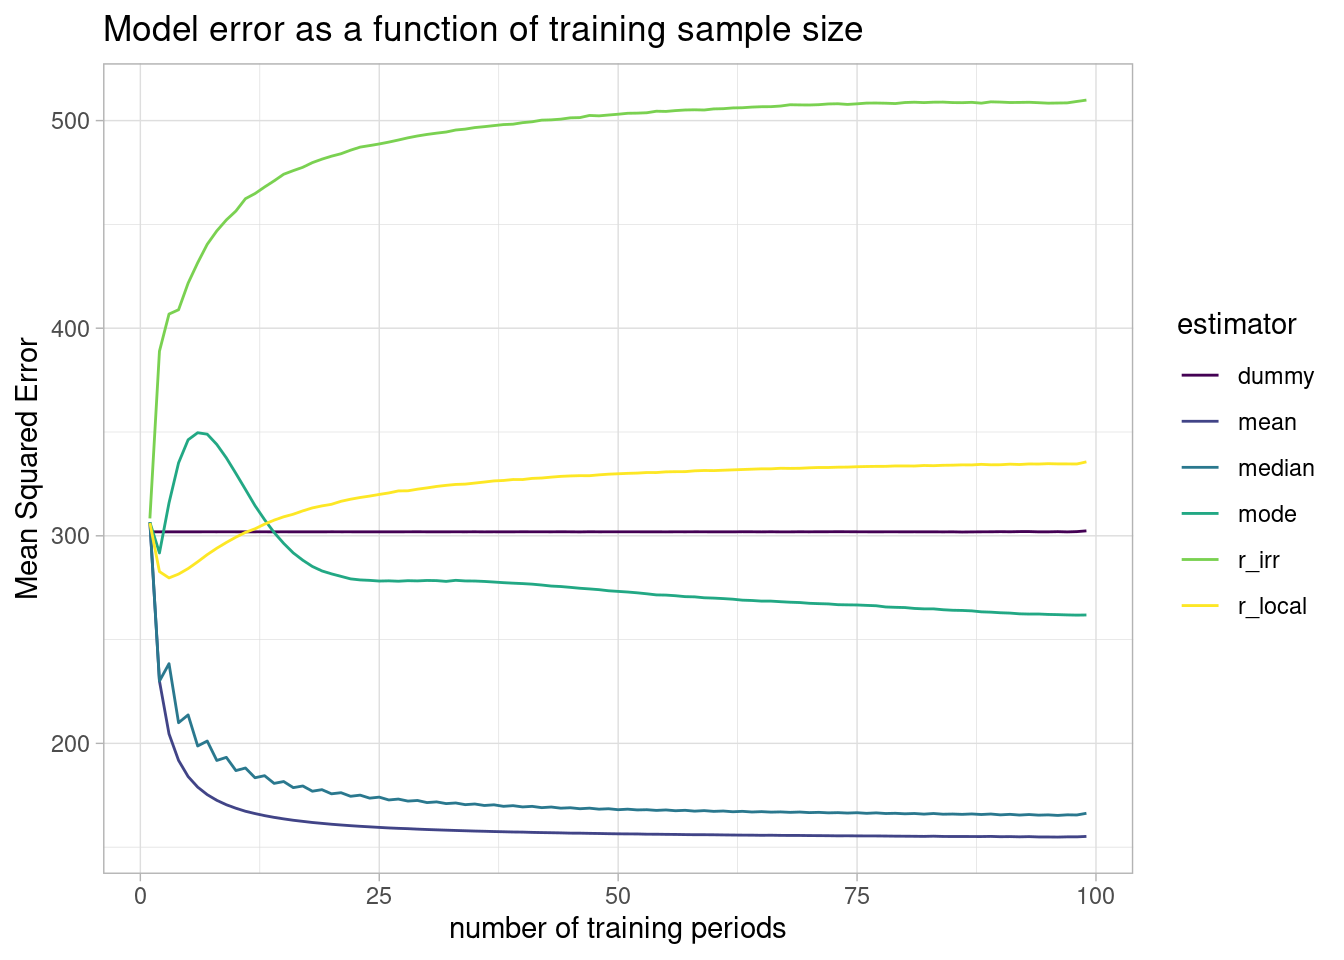
\includegraphics{_main_files/figure-latex/plt-error-model4-1.pdf}
\caption{\label{fig:plt-error-model4}Descriptives power of different models.}
\end{figure}

We see that the models that perform the worst are the models that can be
generalized to other choice sets. The r\_irr model always performs worse
than the dummy model and the r\_local model performs worse as soon as the
number of observations per subject becomes larger than 10. These two
models perform poorer as the number of observations in the learning
sample increases. In general these two models perform worse than the
dummy model and do not seem to be relevant for predicting individual
behavior. The mode-based model performs a little better than the dummy
model when the number of training observations is higher than 14 but
less otherwise. The best performing models are the median- and mean-based
models. Both have a similar behavior in performing better when the
training period is long. In the end, these 2 models perform much better
than the dummy model. The mean-based model performs a little better than
the median-based model. But even with 99 training periods the mean based
model displays an MSE of more than 155.

In order to test the ability of the different models to predict the
future behavior of the subjects, we use a similar approach to the
previous one, but we separate the training and test samples according to
their order. We create a training sample of size m for a subject by
selecting the first m observations. Then we compute the MSE on the next
100-m observations, for each subject. By doing so we effectively test
the ability of the models to predict future behavior by respecting the
serial nature of the data. We can therefore construct a linear regression
model for each subject that includes as an explanatory variable for a
choice the choices made in previous periods. For each subject the model
includes up to the last 5 choices in order to predict the choice of the
current period, note that for some subjects the choices of the previous
periods can be perfectly correlated between them and that in this case
the number of previous choices included is reduced in order not to
include two variables perfectly correlated between them. In order to be
able to compare the performances of the different models we have used in
addition to the linear regression some of the models used previously. In
the figure \ref{fig:dummy-estim4} we present the performance in terms of MSE of
the different models for different learning sample sizes.

\begin{figure}
\centering
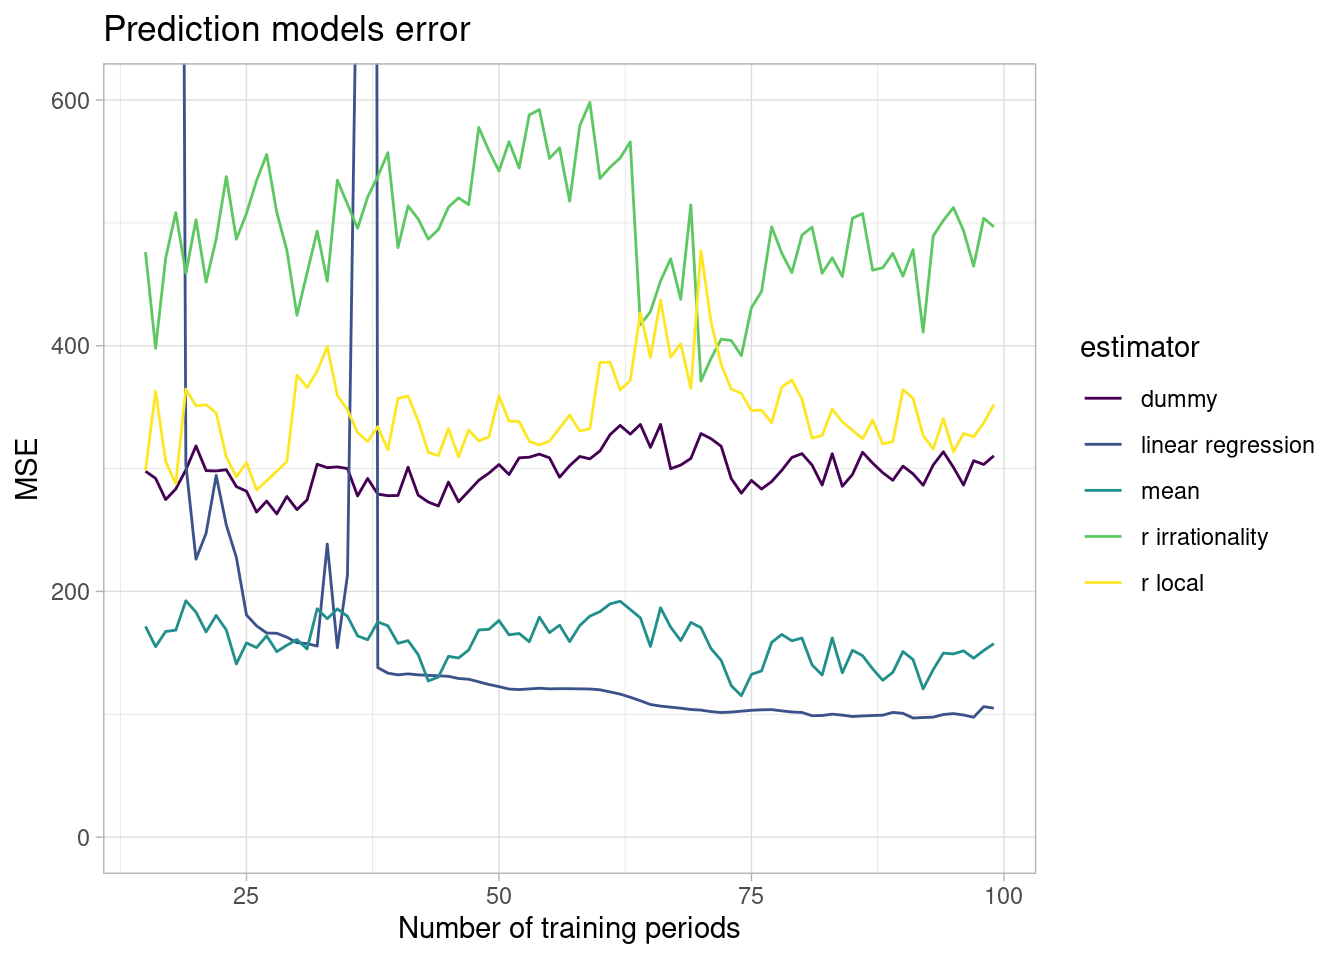
\includegraphics{_main_files/figure-latex/dummy-estim4-1.pdf}
\caption{\label{fig:dummy-estim4}Predictives power of different models.}
\end{figure}

As before, the least efficient models are those based on the calculation
of a risk aversion parameter. This type of model offers a lower
predictive power than the dummy model which always predicts 32. The
mean-based model still offers better results than the dummy model. It is
also the best performing model when the number of observations in the
training sample is low (about less than 40). Finally, the linear
regression model offers extremely variable results for a small number of
observations (about 40) but when the number of observations in the
training sample is sufficient it is this type of model that gives the
best results. Moreover, it seems that the regression model learns more
than the mean-based model when the number of observations increases,
which can lead us to hope that with a larger number of observations we
can obtain good predictions.

By comparing the predictions of linear and mean models, we show the
importance of a subject's previous choices on his decisions. If linear
regressions offer better results it is because in some way the
individual choices are not independent and it is possible to build
models taking into account this dependence. Insofar as the linear
regressions we have built here were built in a rudimentary way and that
no model selection tools or even interaction terms or variables of order
different from 1 were tested, it would be possible to have better
results for this type of model. Another possibility of improvement would
be the use of other classes of models like random forests.

This shows that to predict individual behavior, models based on a risk
aversion parameter perform poorly on the simplest possible task. That
when it comes to summarize these predictions using a single parameter or
when we have few observation, the best parameter are the
average of observations. But that the predictions obtained in this way
are likely to be mediocre. But it should be possible to obtain better
quality predictions if we use the right models and have a large number
of observations.

\hypertarget{discu4}{%
\section{Conclusion}\label{discu4}}

In this article we have tried to provide some answers to the following
question: When an individual is confronted several times with the same
situation, does he always make the same choice? To do this, we proposed
an experimental protocol in which our subjects were repeatedly asked the
same question. The repetitions are done one after the other and the
subjects receive no feedback before the end of the experiment. The question
asked concerns risk preferences. Risk preferences are central to many
decisions and their elicitation has already been widely studied in
experimental economics. We therefore chose to adapt the BART method used
in economics and psychology. This allowed us to repeatedly ask a
question with the following properties:

\begin{enumerate}
\def\labelenumi{\arabic{enumi}.}
\tightlist
\item
  The answer to the question is simple (choose a number between 0 and

  \begin{enumerate}
  \def\labelenumii{\arabic{enumii})}
  \setcounter{enumii}{63}
  \tightlist
  \item
    and fast, especially since the subject chooses to always answer
    in the same way.
  \end{enumerate}
\item
  Subjects are encouraged to answer according to their preferences.
\item
  A subject with fixed preferences is encouraged to answer always in
  the same way.
\item
  The set of possible responses is large and therefore allows for
  variations in responses of different magnitudes.
\end{enumerate}

With this question, we expected subjects to respond in the same way on all
occasions.

But our results show that the subjects act in a varied way and that only
a 6.67\% of them always make
the same choice. So even if the average value chosen by the subjects is
coherent with the literature on the subject, the variability of the
choices is very important between the subjects and high for an important
part of the subjects. We show that this variability in the answers has
important consequences on the modeling and estimation of the preferences
for the risk. First of all, the estimation of a risk aversion parameter
is extremely imprecise with a coefficient of variation for the parameter \(r\) of
roughtly 429 for CRRA function.
The distribution of the answers is not normal for
52.33\% of the subjects
and for 20.67\% of the
subjects we cannot even be confident that their answer can be
described with a central value.

Beyond the theoretical considerations for modeling that our results
raise, we also show that the way individuals choose has practical
consequences both on the methods used in experimental economics to test
hypotheses and on the reliability of the conclusions that can be deduced
from the estimation of a risk aversion parameter. Indeed, our results
show that in a situation of repeated choice with between- or within-subjects
experimental designs the chances of concluding wrongly that there is a
significant effect are significantly higher than the significance threshold chosen for the tests.
The difference-in-difference designs do not seem to suffer from this
effect. We also show that the correlation of risk aversion measures for
the same task is only about
0.4.
This value is much lower than what one would expect (a correlation of 1)
and may explain the low level of correlation observed between the
various methods of measuring risk preferences. Moreover, we show that
models based on the evaluation of a risk aversion parameter that can be
generalized to different sets are very poor models for describing
individual behavior. The best alternative to describe individual
behaviors with a parameter is to use the mean observation. This
paradoxical conclusion with our first conclusion led us to test an
alternative model, individual linear regression. We compared this new
model with the others according to their predictive power. We show that
the predictive power of models based on a risk aversion parameter is as
bad as their descriptive power. But we also show that when the number of
observations is sufficient, the model based on linear regressions
provides better results than the average. This shows us that it is easy to
achieve better results than those proposed by the economic models.

Our results suggest that a static model based on a risk aversion
parameter is not suitable to describe individual behavior. Indeed, we
have shown that this type of model obtains poor results both from a
descriptive and predictive point of view even in the simplest task. This
is consistent with the work of \citet{wilcox2007predicting} which shows the
weaknesses of this type of model in a slightly more complex task.
However, it seems possible to learn more about individual behavior by
having enough observations on repeated choices to train statistical
models that could highlight behavioral regularities.

Finally, we can answer our question by saying that the elements at our
disposal lead us to say that confronted with the same situation several
times, individuals will act in different ways. But this question would
deserve more work and results than the few elements we have brought
here.

\hypertarget{conclusion5}{%
\chapter{Conclusion}\label{conclusion5}}

This thesis has been for me the opportunity to shape my understanding of
economic research;
in particular the impact of different approaches to experiments in economics.
When I started my thesis, I was focused on developing experimental protocols
that would allow me to measure subjects' preferences as accurately as possible.
To design these protocols I relied heavily on theoretical work concerning the
models I wanted to test.
My goal was to place my subjects in a situation as close as possible to the
theoretical model while exploring as much as possible the impact of the
different parameters of the model on individual preferences.
The experiment presented in chapter 2 is an example of this approach and it
suffers from this approach which limits the robustness of the analysis of the
data in this chapter.
My collaboration with Rustam Romaniuc, Dimitri Dubois and Paolo Crosetto
encouraged me to develop an experimental protocol for the temptation model of
\citet{gul2001temptation} but which aimed at highlighting the demand for commitment and
the capacity of individuals to exercise self-control.
This approach that tests the behavioral predictions of the models is the common
approach in the literature.
This approach allows to document the specificities of individual behaviors
and thus guide the development of theories.
But identifying behaviors consistent with a theory does not test its validity.
As pointed out by Karl Popper in \citet{popper2005logic} a given behavior can be
predicted by a large number of different models, he also underlines the
asymmetry between confirmation and denial of a theory.
No matter how many observations in favor of a theory we have, it only takes one
observation to invalidate it.
This must however be relativized by the imprecision and the possible errors of
observations.
But this idea encouraged me to adopt a different approach from the standard
approach in experimental economics in the second half of my thesis.
The idea is to construct the experimental protocol in such a way as to
repeatedly observe a situation in which we know the theoretically expected
behavior.
We then compare the observed behavior to the behavior predicted by one or more
theories.
This approach, even if it does not allow us to falsify a theory in the sense of
Karl Popper, allows us to compare different models.

By applying this approach and comparing economic models to simple statistical
models I have shown in this thesis that the temptation model proposed by
\citet{gul2001temptation} predicts behaviors that are actually observed in our
experience.
This model represents a more accurate description of subjects' choices for menus
than the standard expected utility model.
But \citet{gul2001temptation}'s model does not describe behaviors more accurately than
a model that ignores the composition of a menu.
This lack of descriptive and predictive ability is also found with the
expectation utility model for lottery choices.
It has been shown that individual choices in the area of risk preferences are
highly variable.
We have also shown that even if the expected utility models and the
\citet{gul2001temptation} model do not correctly account for the choices of the
subjects, it is possible to propose models that better describe the individual
choices than the constant response models that equalize our economic models.

To conclude, I would like to propose an interesting way to improve risk
preference models.
The idea comes from the foreword \citet{aliprantis2006hitchhiker}
``It has become clear in the last couple of decades that eco-
nomic models capable of addressing real policy questions must be both stochastic
and dynamic. There are fundamental aspects of the economy that static mod-
els cannot capture. Deterministic models, even chaotically deterministic models,
seem unable to explain our observations of the world.''.
I think that looking for models that allow individual choices to be both dynamic
and random could improve the predictive and descriptive capacity of models in
economics.

\hypertarget{references}{%
\chapter*{References}\label{references}}
\addcontentsline{toc}{chapter}{References}

\hypertarget{refs}{}
\begin{CSLReferences}{0}{0}
\end{CSLReferences}

\hypertarget{appendix-appendix}{%
\appendix}


\hypertarget{experimental-instruction-for-chapter-2}{%
\chapter{Experimental instruction for chapter 2}\label{experimental-instruction-for-chapter-2}}

This will be Appendix A.

\hypertarget{experimental-instruction-for-chapter-3}{%
\chapter{Experimental instruction for chapter 3}\label{experimental-instruction-for-chapter-3}}

This will be Appendix B.

\hypertarget{experimental-instruction-for-chapter-4}{%
\chapter{Experimental instruction for chapter 4}\label{experimental-instruction-for-chapter-4}}

  \bibliography{bibliography.bib}

\end{document}
